\documentclass{article}
%\documentclass[journal,transmag]{IEEEtran}
%\documentclass[10pt, conference]{IEEEtran}
\usepackage{amsmath}
\usepackage{graphicx}
%\usepackage{listings}
%\usepackage{circuitikz}
\usepackage{lscape}
\usepackage{ulem}
\usepackage{float}


\usepackage[scale=0.8]{geometry}
\begin{document}

\title{E6312: Problem Set 2}
\author{Miles Sherman}
\date{\today}
\maketitle

\textit{In the previous problem set, I measured various behaviors of the MOSFET transistor at the 180nm technology node. I mostly made direct measurements on input and output voltages as well as currents in an effort to better understand the different regions of operation of the devices. In this problem set, I take a first step towards measurement of parasitics in the devices by looking at intrinsic capacitances. In addition, I will build three basic amplifiers and measure their performance.}

\section{Problem 1: Intrinsic Capacitances}
\subsection{$C_{gs}$}
I measured the values for the gate to source capacitance using both DC operating point simulation as well as AC Analysis. To acquire the necessary DC operating simulation I first constructed the circuit shown in Figure \ref{1_dc_schem}. This circuit allows utilizes an nMOS transistor with $W/L = 1\mu m/180nm$. I ran a DC simulation on the circuit sweeping $V_{DS}$ from 0V to 1.8V and outputting drain current with $V_{GS}$ = 0.8V. Using the results browser I then plotted $C_{gs}$ (minus $C_{gs-overlap}$) against $V_{DS}$ (Figure \ref{1a}).

My next step was to attempt to attain the same measurements of $C_{gs}$ using the method of AC analysis. To do this, I began by constructing the circuit shown in Figure \ref{1_ac_schem} (note that the two AC voltage sources are toggled on/off in the simulating environment). My goal in this simulation was to isolate $C_{gs}$ and utilize the capacitance equation
\begin{equation}
C = \frac{i_c}{2\pi fv_c}
\end{equation}
to plot $C_{gs}$. I applied an AC signal of 10mV amplitude and low frequency to the source of the device. I then plotted the current into the gate of the device while sweeping $V_{DS}$. Even though the current at the gate flows to $C_{gs}$ and $C_{gd}$, because the AC voltage is on the source, AC current flows through $C_{gs}$ but not $C_{gd}$. Utilizing equation 1 as well as the overlap capacitance which was acquired from the results browser, I was able to plot $C_{gs}$ against $V_{DS}$ (Figure \ref{1d}). As is expected in both of my plots, $C_{gs}$ begins at approximately $C_{OX}/2$ ($C_{OX} ~= 1.5fF$). However, one would expect the plots to saturate at $\frac{2}{3} C_{OX}$ for values of $V_{DS}$ greater than $V_{DS-SAT}$. This is not the case in my plots and I attribute this to short-comings in the model file.

\begin{figure}[H]
\centering
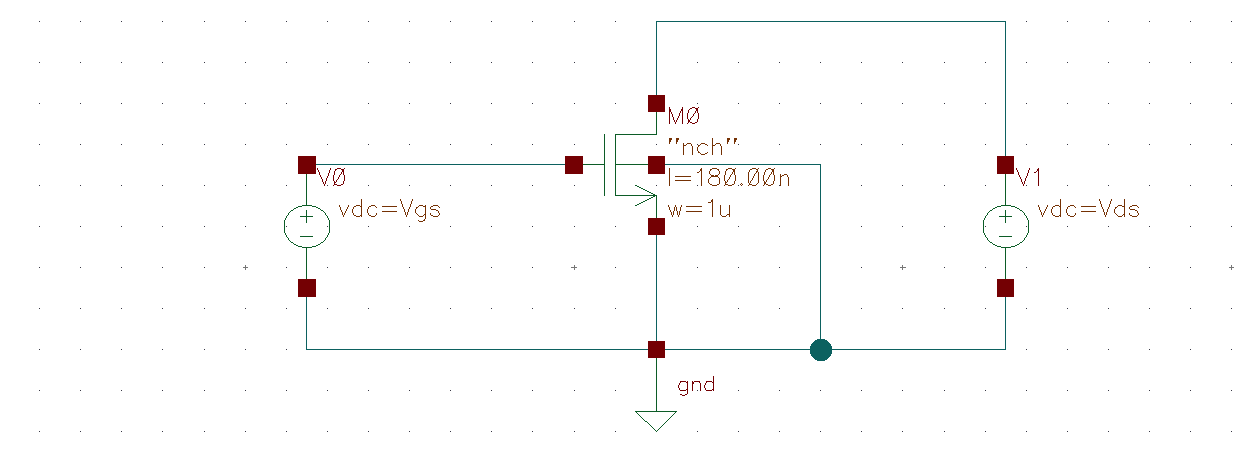
\includegraphics[width=7in]{1_dc_schematic.png}
\caption{Schematic to Simulate DC Operating Point}
\label{1_dc_schem}
\end{figure}

\begin{figure}[H]
\centering
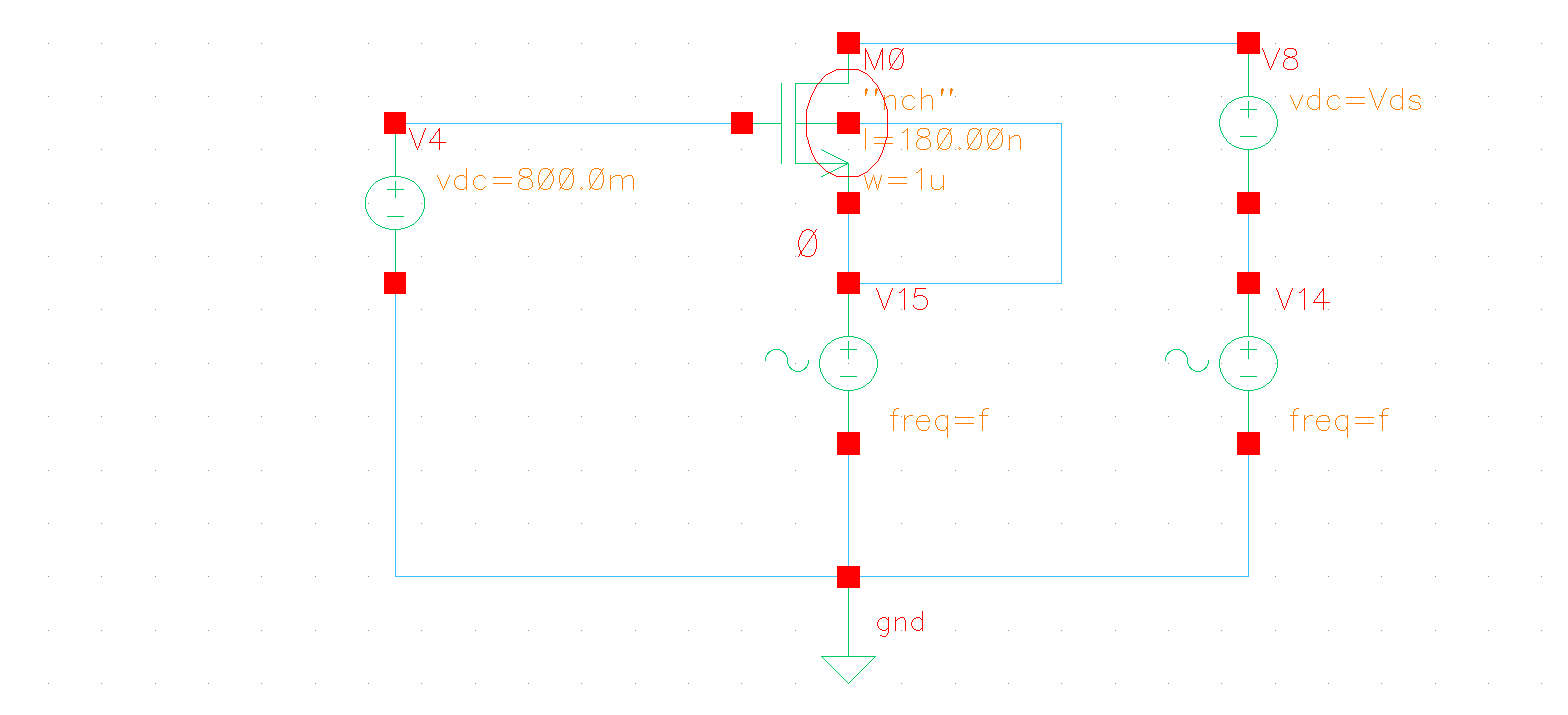
\includegraphics[width=7in]{1_ac_schematic.png}
\caption{Schematic to Simulate AC Operation}
\label{1_ac_schem}
\end{figure}

\begin{figure}[H]
\centering
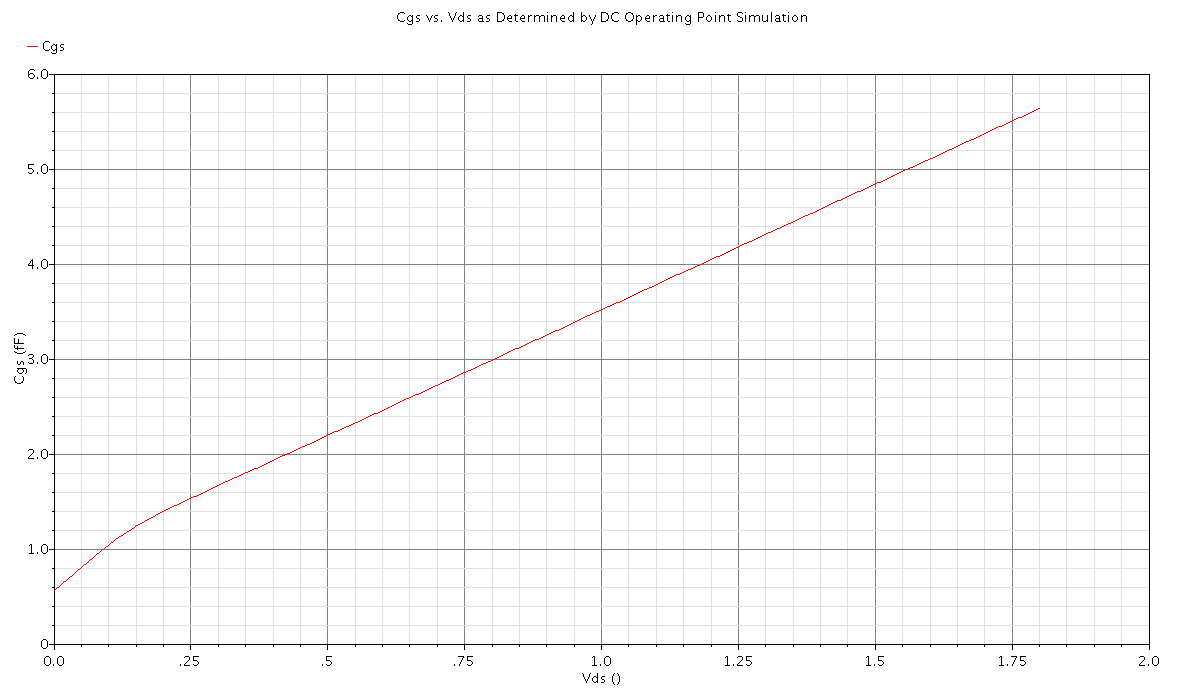
\includegraphics[width=5in]{1a.png}
\caption{$C_{gs}$ vs. $V_{DS}$ as Determined by DC Operating Point Simulation}
\label{1a}
\end{figure}

\begin{figure}[H]
\centering
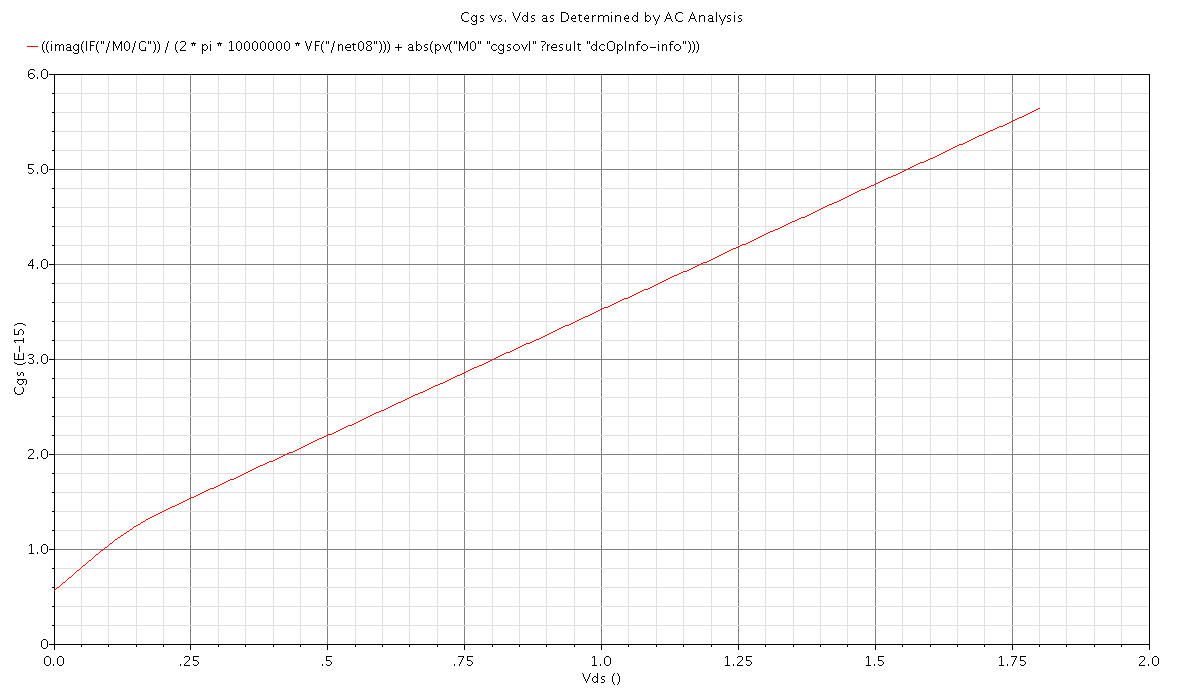
\includegraphics[width=5in]{1d.png}
\caption{$C_{gs}$ vs. $V_{DS}$ as Determined by AC Analysis}
\label{1d}
\end{figure}
\newpage

\subsection{$C_{gd}$}
To measure $C_{gd}$, I performed almost identical simulations to those of $C_{gs}$. However, to plot $C_{gd}$ using AC analysis, I applied an AC signal to the drain of the device instead of the source and simulated current into the gate. This has the same isolating effect but this time on $C_{gd}$ instead of $C_{gs}$. My plots can be seen in Figure \ref{1b} and Figure \ref{1e} (note that in these plots I also had to eliminate overlap capacitance which was acquired from the results browser. $C_{gd}$ begins at $C_{OX}/2$, drops steadily, and then saturates to about 0F at $V_{DS-SAT}$.

\begin{figure}[H]
\centering
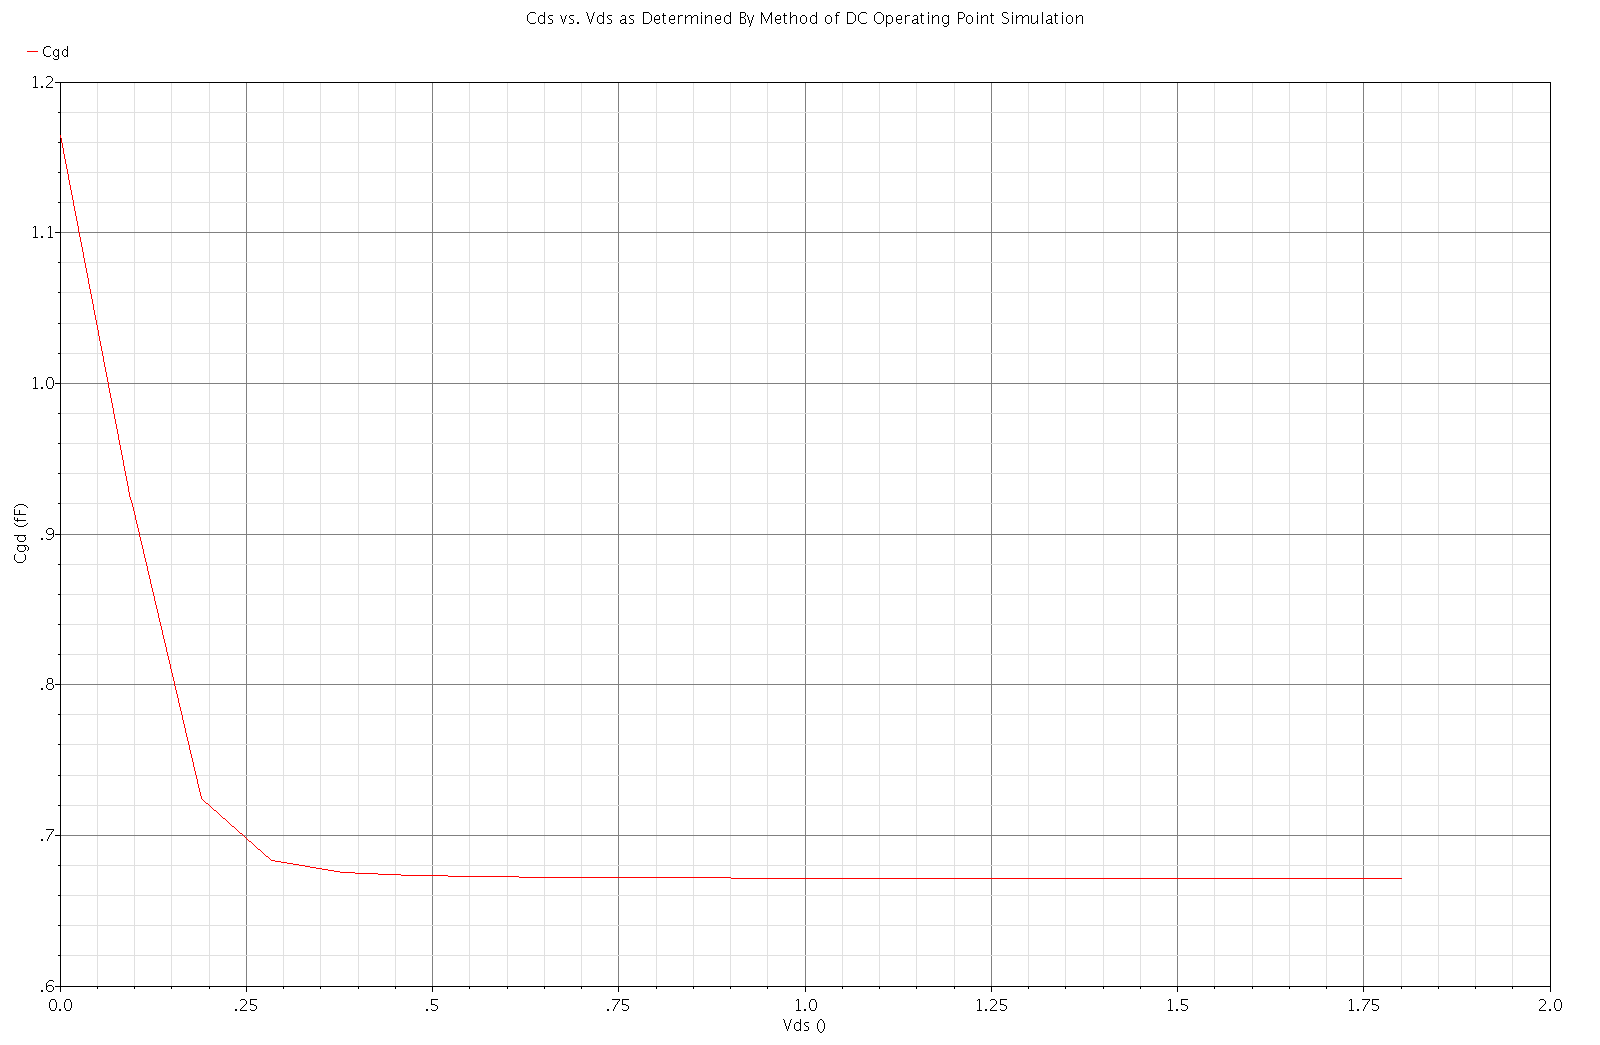
\includegraphics[width=5in]{1b.png}
\caption{$C_{gd}$ vs. $V_{DS}$ as Determined by DC Operating Point Simulation}
\label{1b}
\end{figure}

\begin{figure}[H]
\centering
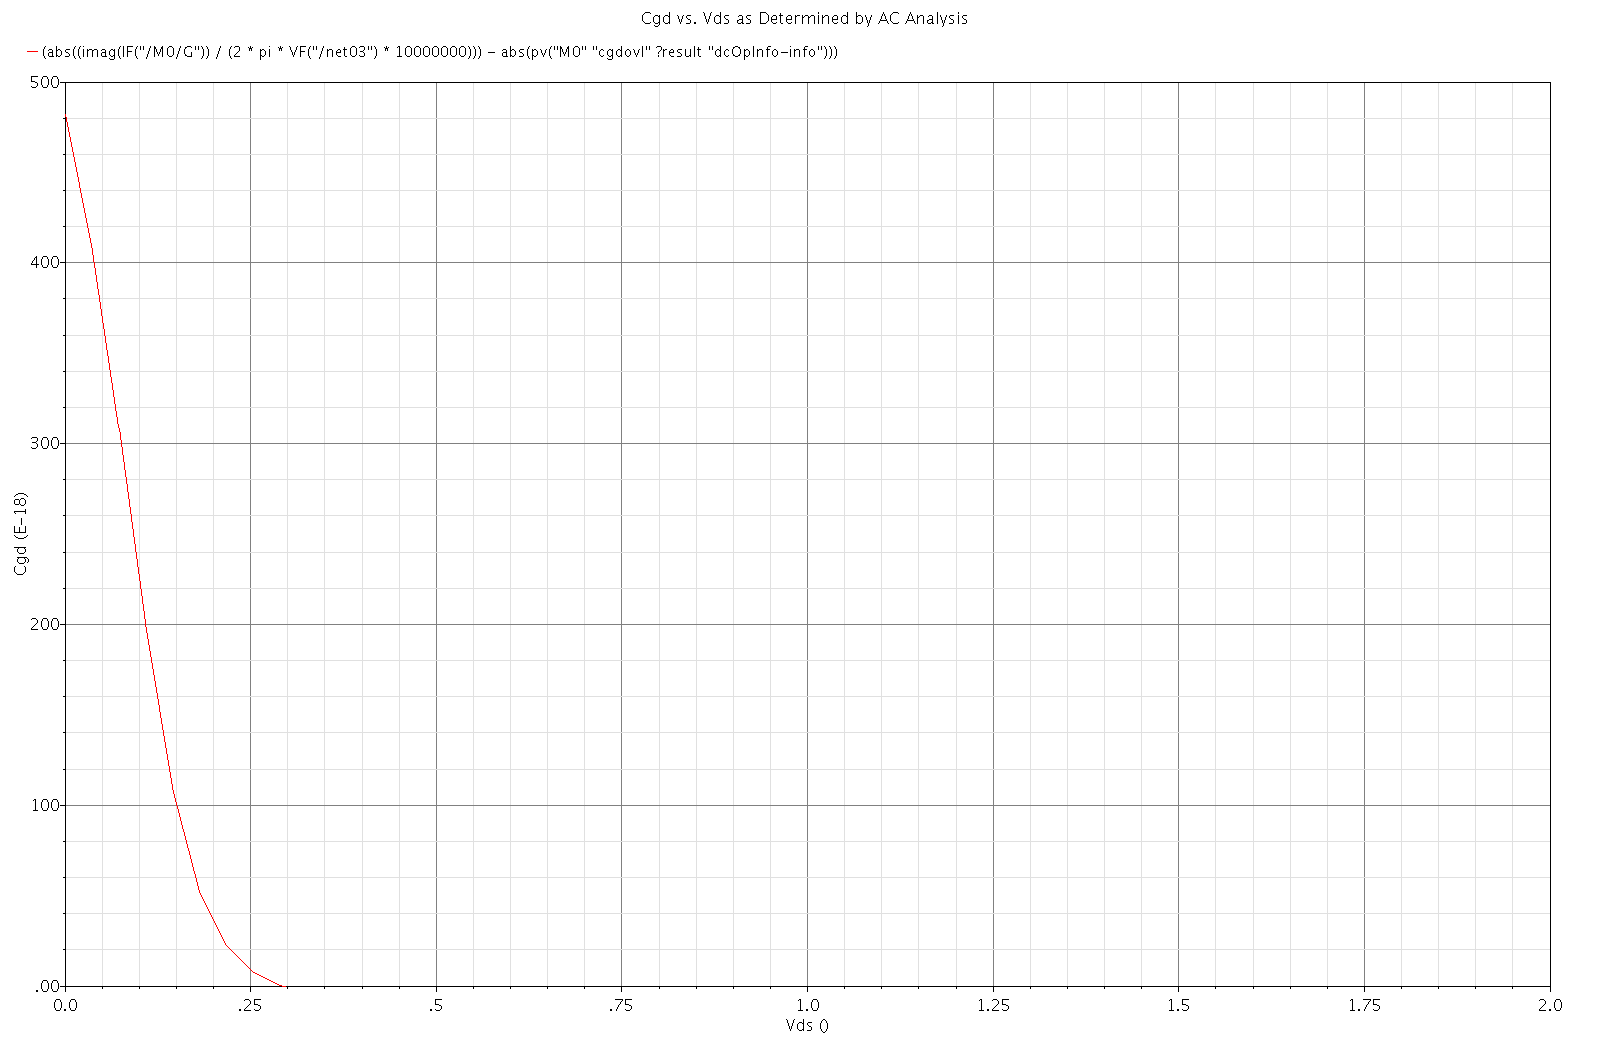
\includegraphics[width=5in]{1e.png}
\caption{$C_{gd}$ vs. $V_{DS}$ as Determined by AC Analysis}
\label{1e}
\end{figure}
\newpage

\subsection{$C_{db}$}
To measure $C_{db}$, I again performed similar DC and AC simulations on my circuit. To simulate the circuit for AC analysis I measured the current into the drain while actually applying an alternating signal to the body. My plots can be seen in Figure \ref{1c} and Figure \ref{1f}.

\begin{figure}[H]
\centering
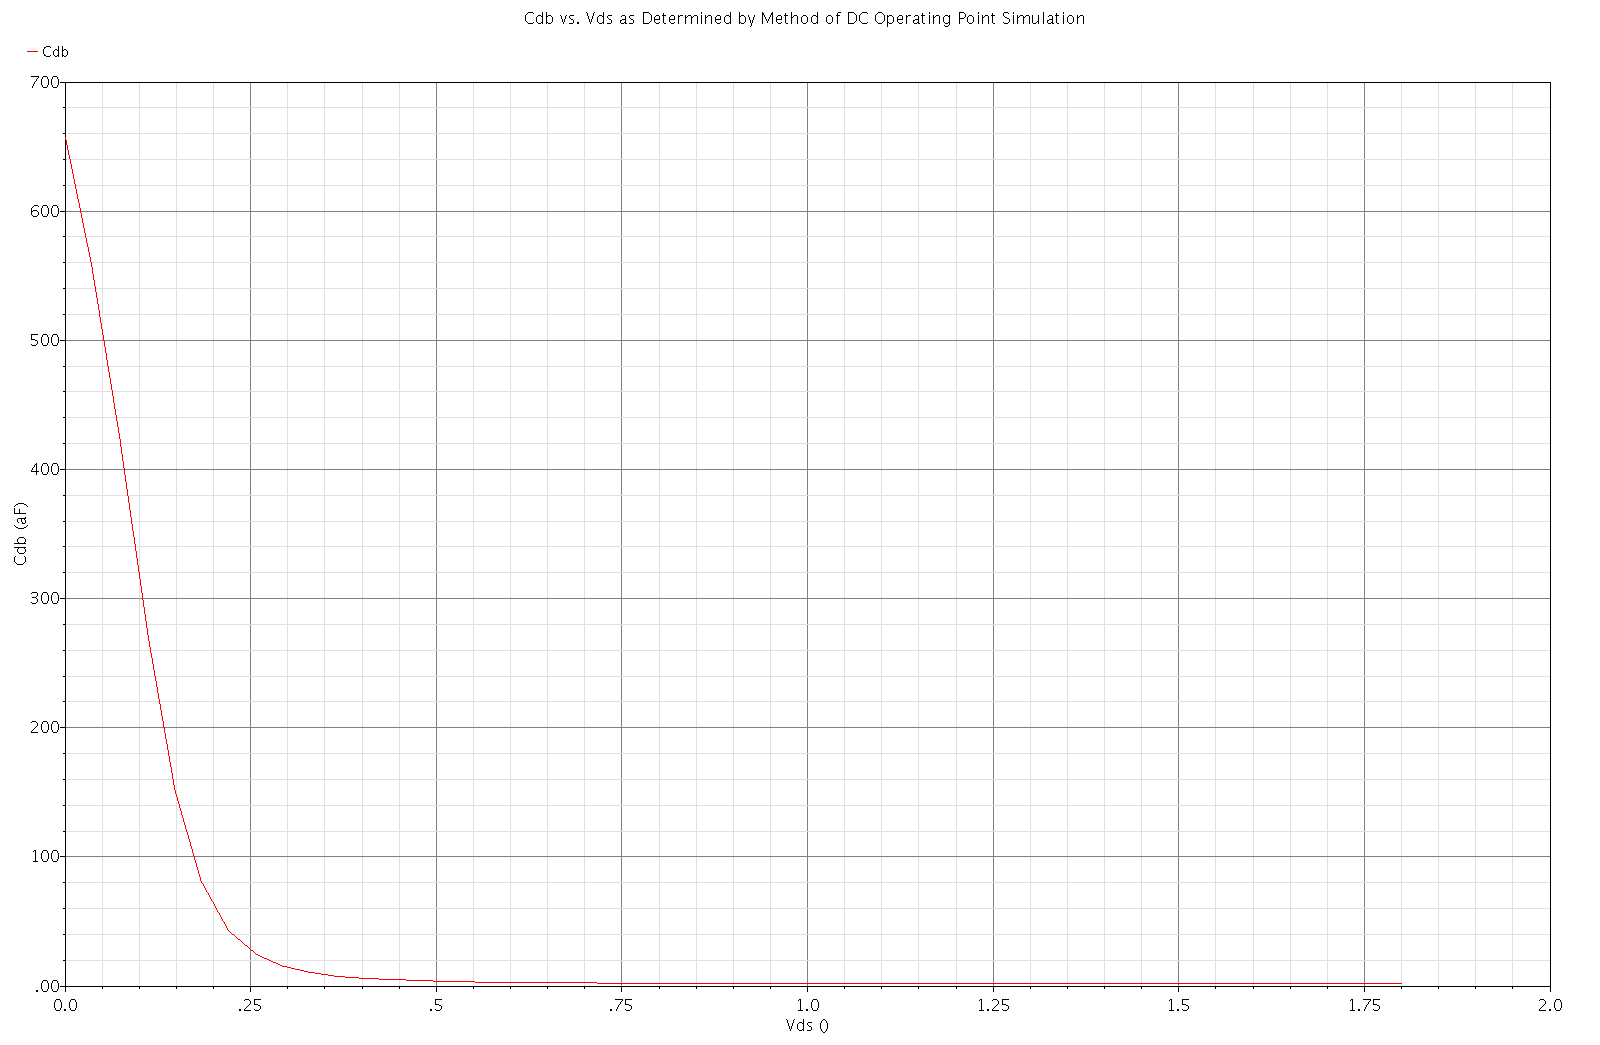
\includegraphics[width=5in]{1c.png}
\caption{$C_{db}$ vs. $V_{DS}$ as Determined by DC Operating Point Simulation}
\label{1c}
\end{figure}

\begin{figure}[H]
\centering
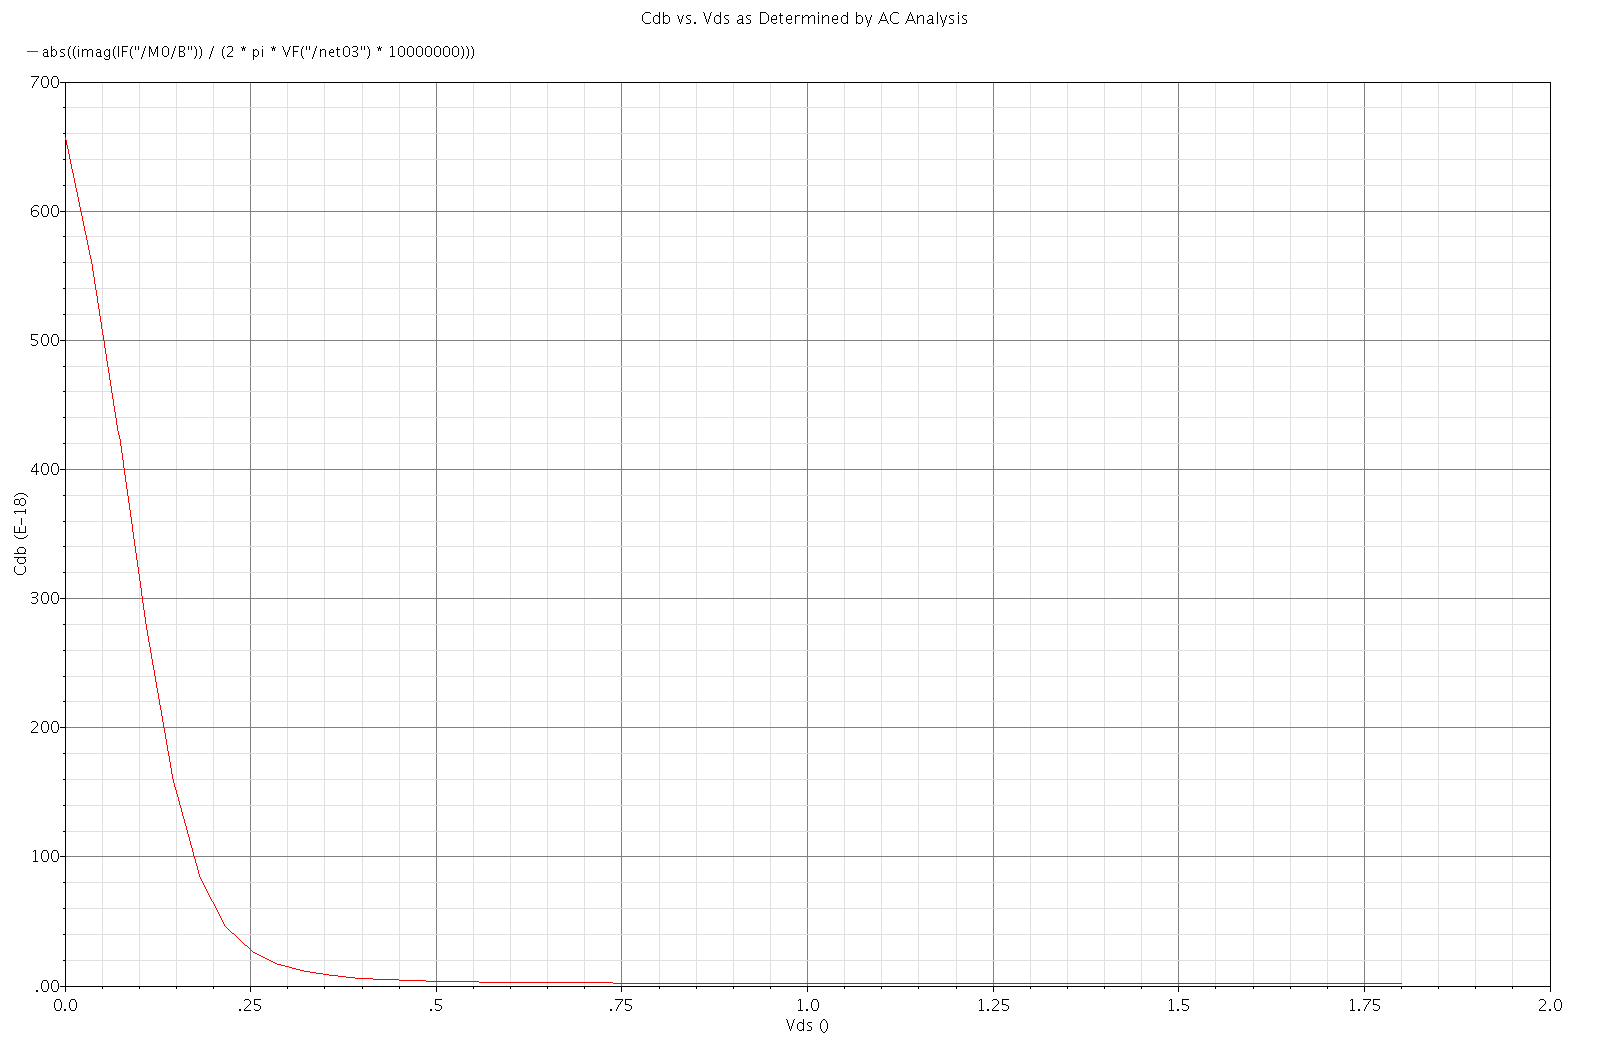
\includegraphics[width=5in]{1f.png}
\caption{$C_{db}$ vs. $V_{DS}$ as Determined by AC Analysis}
\label{1f}
\end{figure}
\newpage

\section{Problem 2: Basic Amplifiers}
\subsection{Common-Source}
For the first part of this problem, I designed a common source amplifier and all associated biasing circuitry. I began by placing my amplifier device as well as unsized placements of my current mirror devices. In order to achieve the maximum output voltage swing, I knew my goal was to set $V_{DS}$ of my amplifier device to approximately 0.9V (halfway between ground and $V_{dd}$). This also would ensure my device to stay in saturation. To achieve this voltage, I sized my current mirror devices appropriately until I observed $V_{DS} = 935.6mV$. Next I chose a value of $V_{GS}$ of 0.7V to bring the device into strong inversion. Because it was readily available from my previous design efforts, I simply connects the gate of my amplifier device to a node of my biasing circuit through a resistor. This brought my $V_{GS}$ to 574.1mV which was acceptable for my purposes. My final design step was to add a small signal source which I connected to the gate of my amplifier device through a large isolating capacitor. The capacitor prevents my small signal source from affecting the biasing of my amplifier. I noted that after the design was complete, $I_{DS}$ of my amplifier device was $17.38\mu A$. My final topology can be seen in Figure \ref{cs_schem} with annotated component parameters and Figure \ref{cs_dcop} with annotated DC operating point.

My next step was to analyze the performance of my circuit as three PVT corners. In the typical case (tt: typical corner, $27^oC$, $V_{dd} = 1.8V$, my low frequency gain was 32.61dB. In the best case (ff: fast corner, $-20^oC$, $V_{dd} = 2.0V$), my low frequency gain was 32.68dB. In the worst case (ss: slow corner, $85^oC$, $V_{dd} = 1.6V$), my low frequency gain was 29.41dB. This was the most steady performance across PVT variations I could achieve. Frequency response plots of these three cases can be seen in Figure \ref{cs_tt}, Figure \ref{cs_ff}, and Figure \ref{cs_ss} respectively.

I calculated the gain of my circuit by hand based on the simulated values of $g_m$ and $r_o$ (for both M0 and M2) using the equation
\begin{equation}
a = g_m(r_{o0} || r_{o2}).
\end{equation}
The result of my hand calculation was $a = 43.08\frac{V}{V}$ or in decibels $a = 32.68dB$. This is a comparable value to my simulated gain.

\begin{figure}[H]
\centering
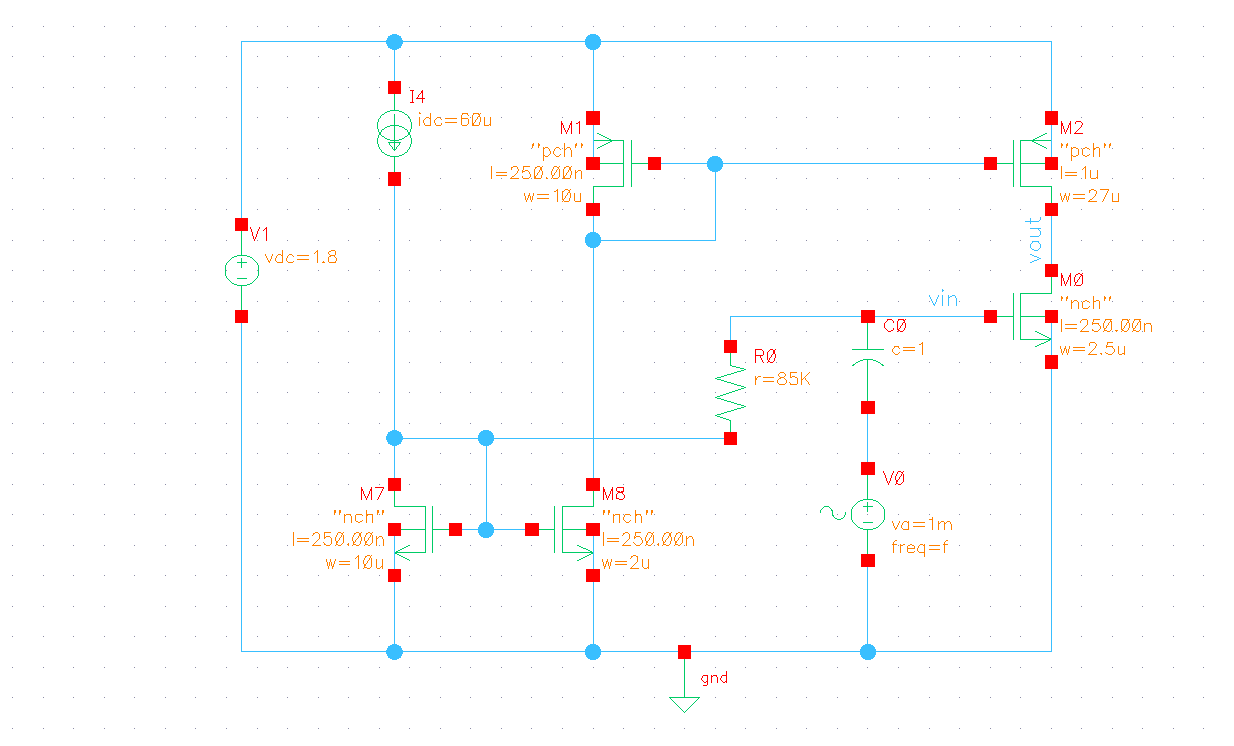
\includegraphics[width=7in]{2_cs_schematic.png}
\caption{Schematic of Common Source Amplifier and Associated Biasing Circuitry}
\label{cs_schem}
\end{figure}

\begin{figure}[H]
\centering
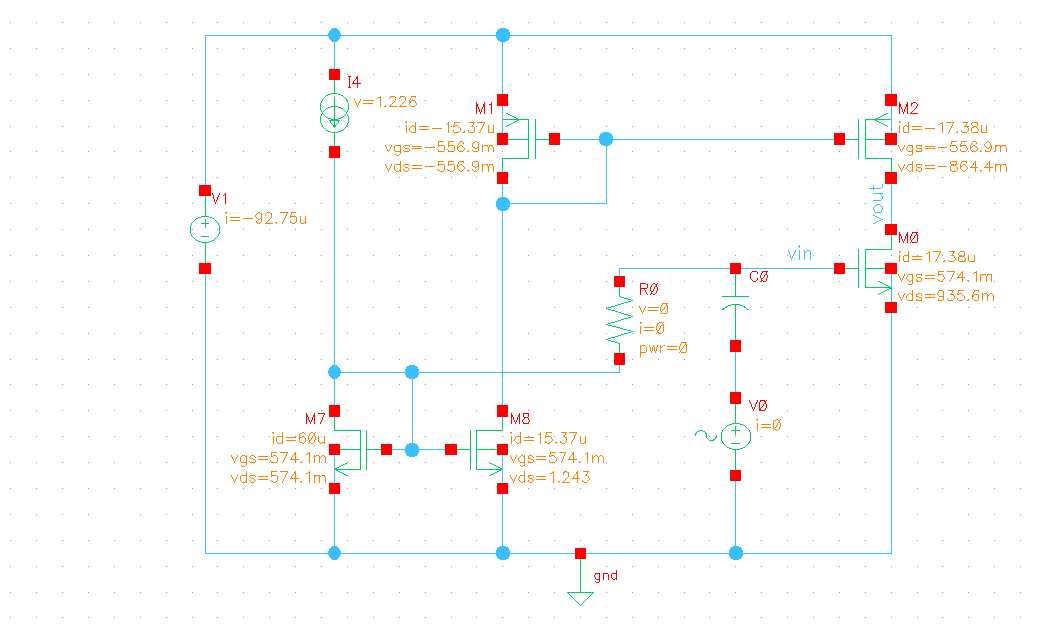
\includegraphics[width=7in]{2_cs_dcop.png}
\caption{Schematic of Common Source Amplifier with DC Operating Point Annotations}
\label{cs_dcop}
\end{figure}

\begin{figure}[H]
\centering
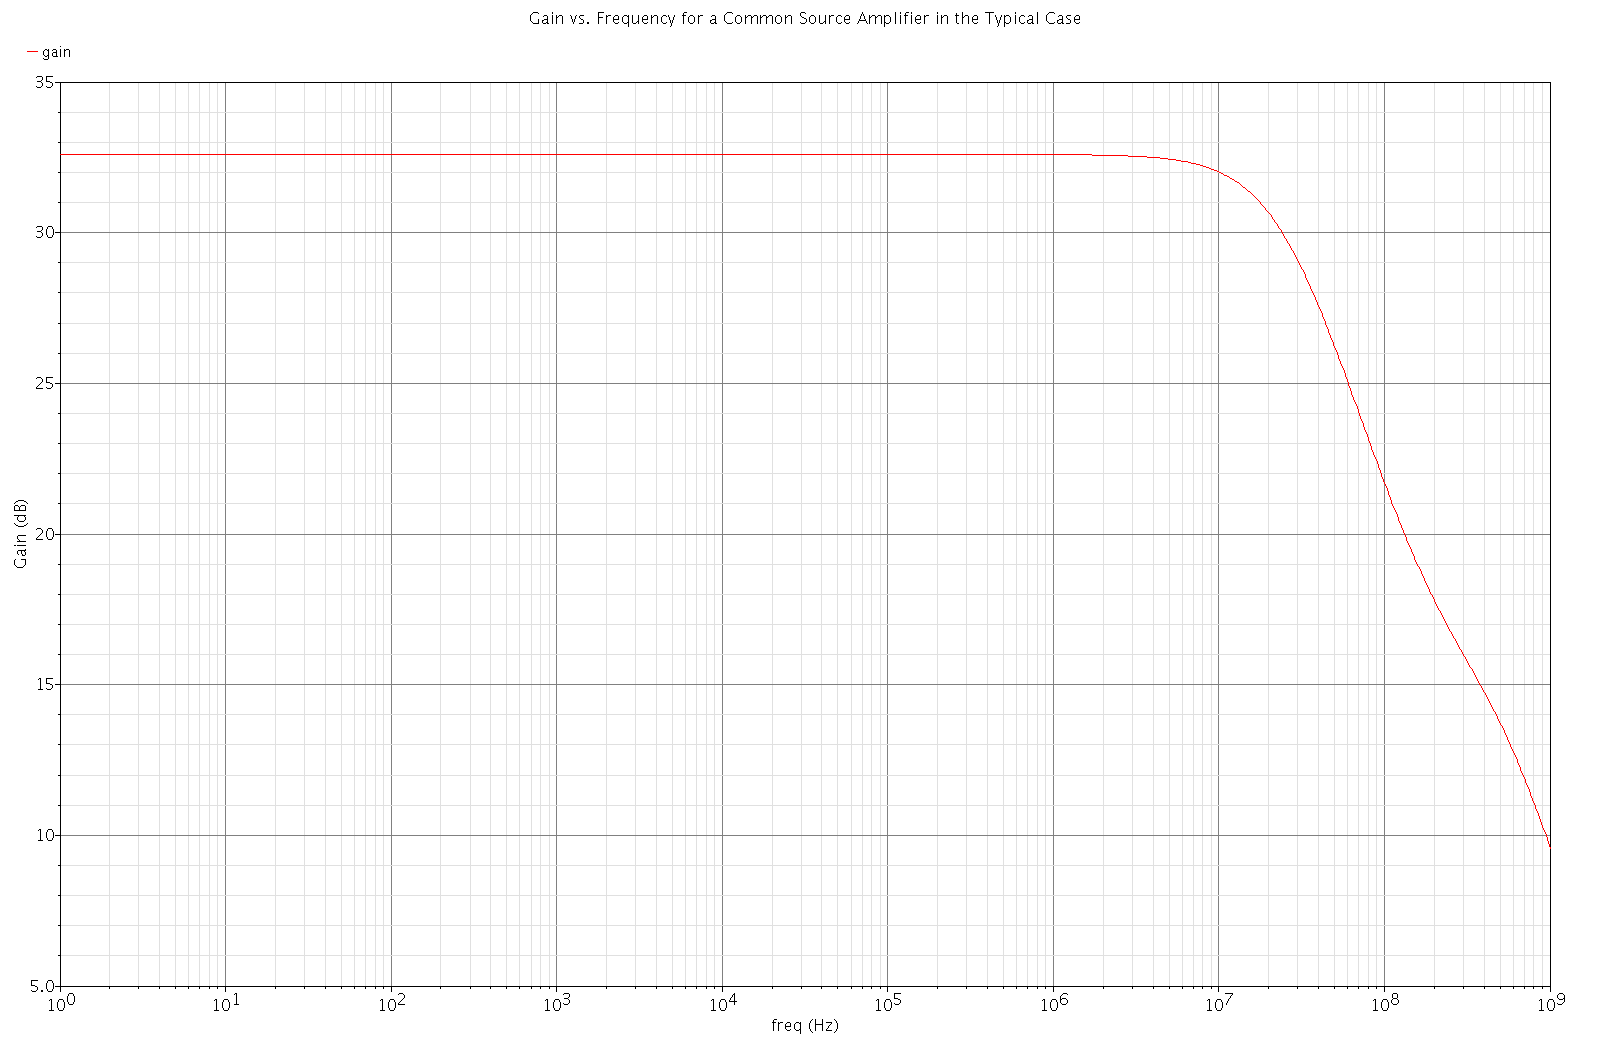
\includegraphics[width=5in]{2_cs_gain_tt.png}
\caption{Frequency Gain of Common Source Amplifier in the Typical Case}
\label{cs_tt}
\end{figure}

\begin{figure}[H]
\centering
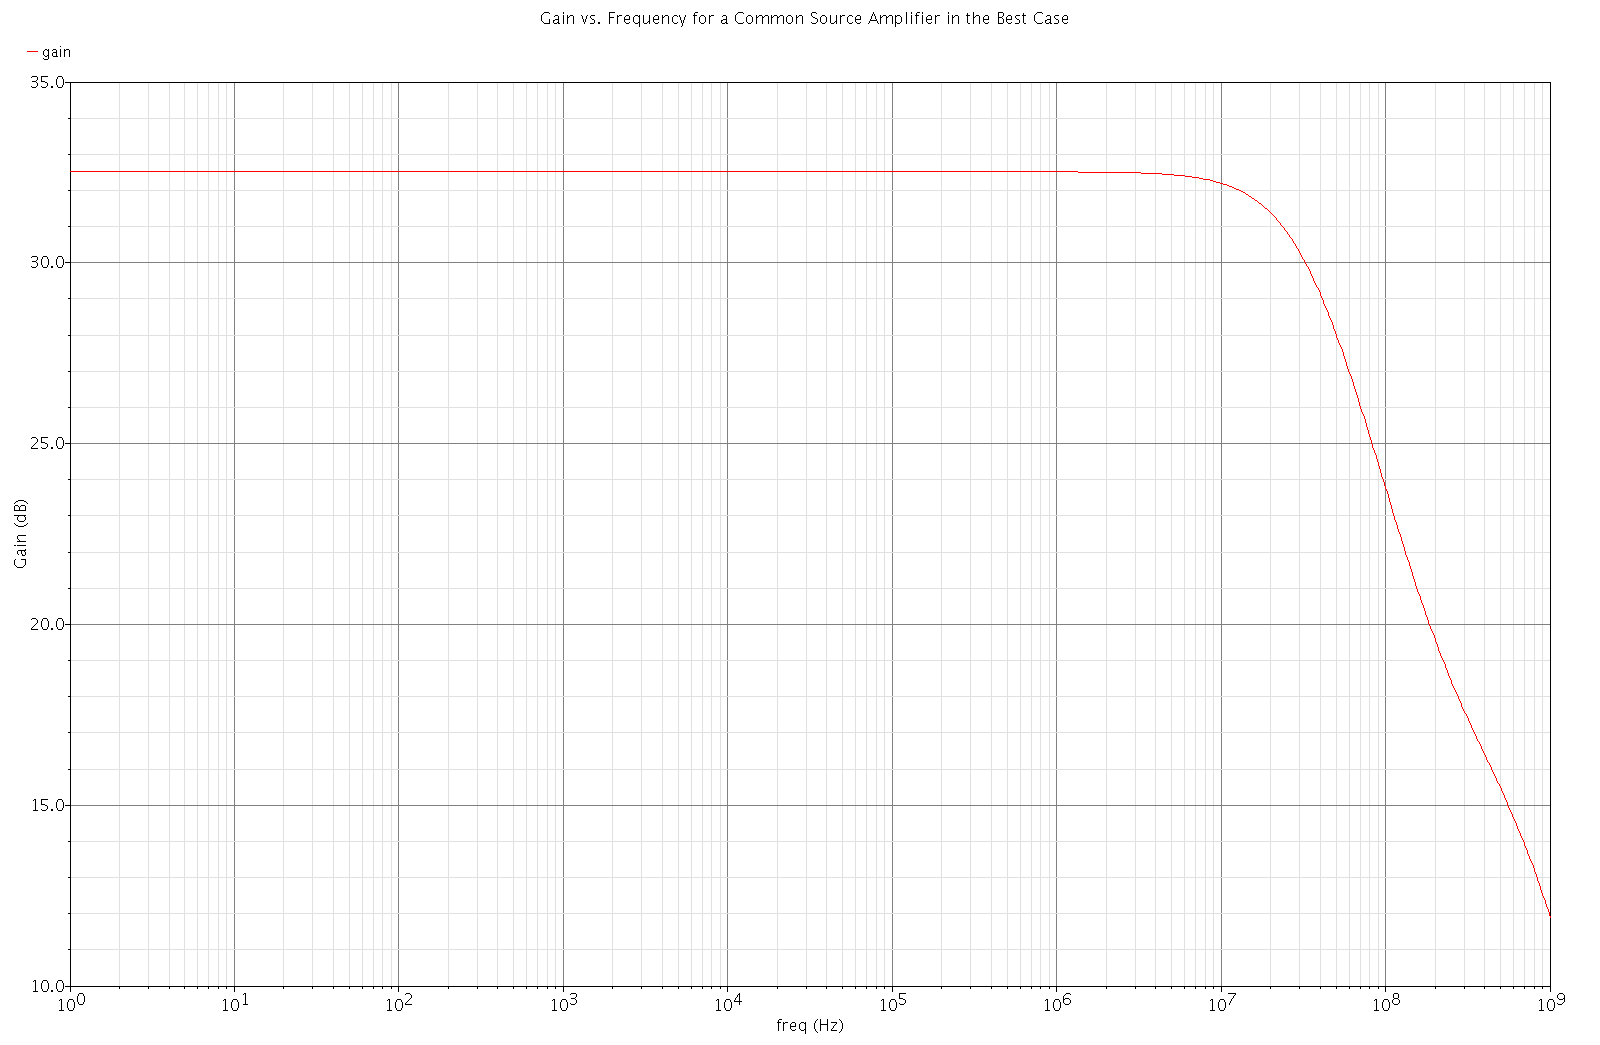
\includegraphics[width=6in]{2_cs_gain_ff.png}
\caption{Frequency Gain of Common Source Amplifier in the Best Case}
\label{cs_ff}
\end{figure}

\begin{figure}[H]
\centering
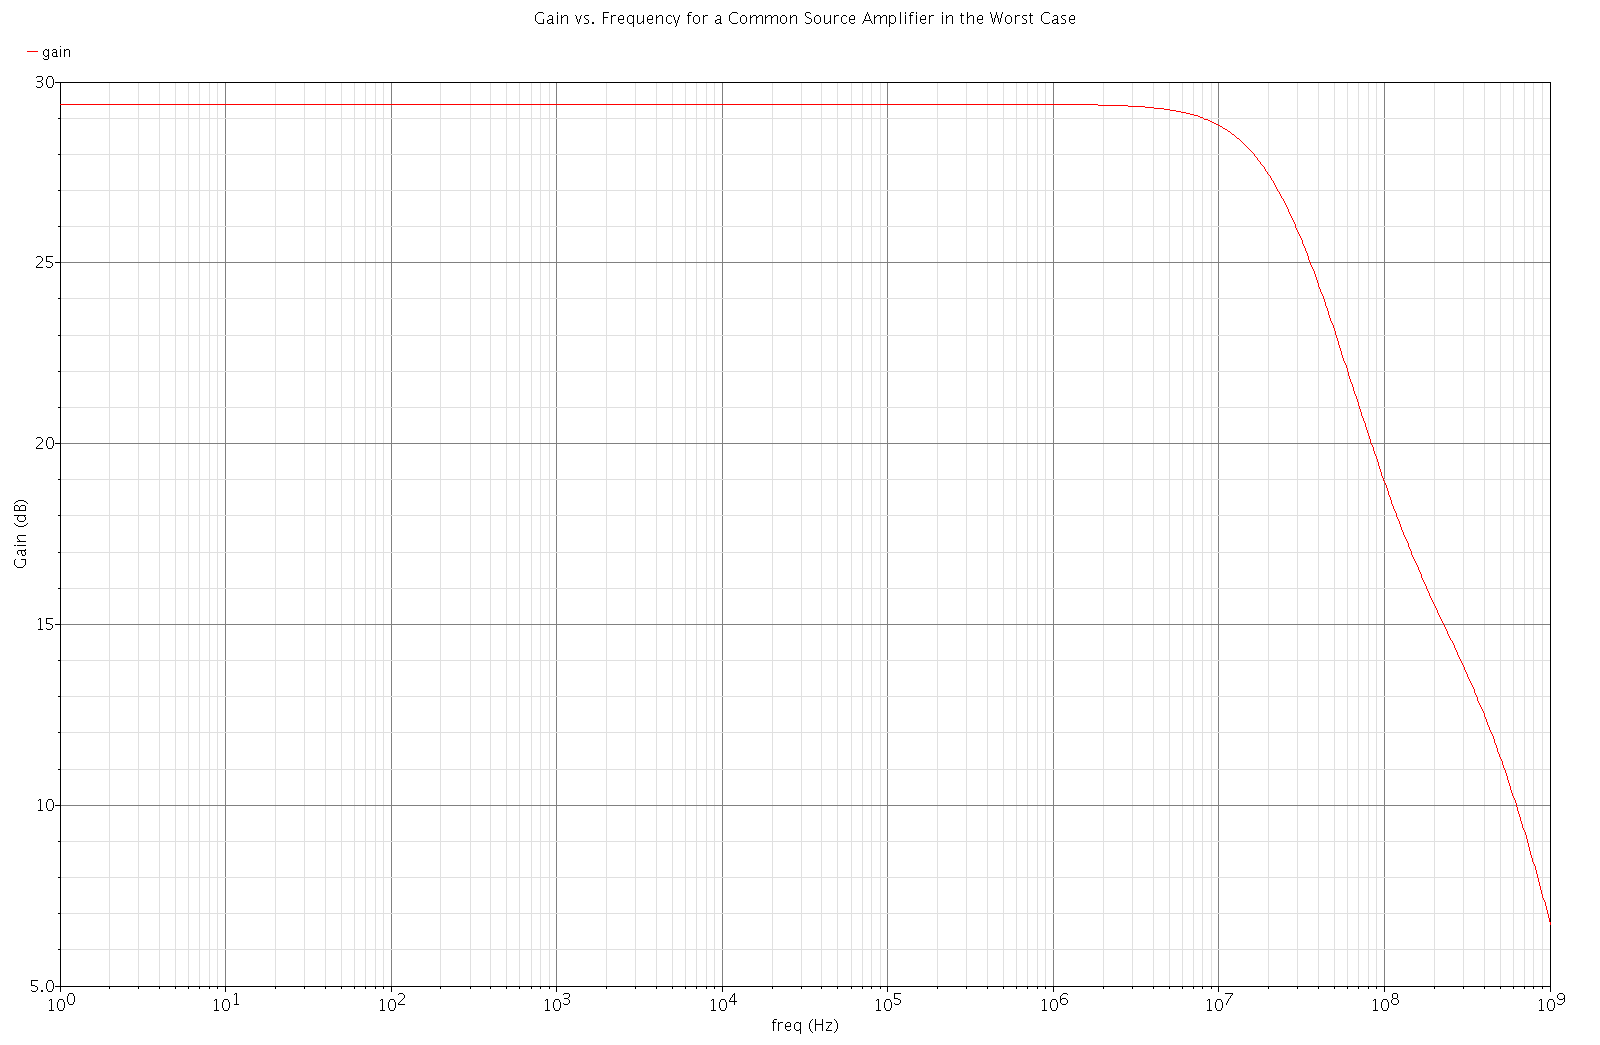
\includegraphics[width=6in]{2_cs_gain_ss.png}
\caption{Frequency Gain of Common Source Amplifier in the Worst Case}
\label{cs_ss}
\end{figure}

My final performance analysis task was to find the maximum input and output voltage swing. To do this I applied a small signal to the gate of the amplifier device at 1MHz and varied its amplitude. I plotted various transient responses on AC input voltage amplitudes between $20mV_{pp}$ and $50mV_{pp}$. As can be seen in Figure \ref{cs_tran}, the output begins to distort for larger amplitudes in the range. To determine the exact input voltage amplitude corresponding to -1dB of distortion, I used the calculator to plot an AC transfer function ($v_{out}$ vs. $v_{in}$). On this same plot, I also plotted a perfectly linear response if the amplifier had a gain of 31.61dB (-1dB). This can be seen in Figure \ref{cs_lin}. The intersection of these two curves shows the maximum input and output voltages (note that the plot shows amplitude from AC ground, not peak-to-peak). My final value of maximum input voltage for linear operation was $v_{in} = 36.56mV_{pp}$ with a corresponding output value of $v_{out} = 1.374V_{pp}$.

\begin{figure}[H]
\centering
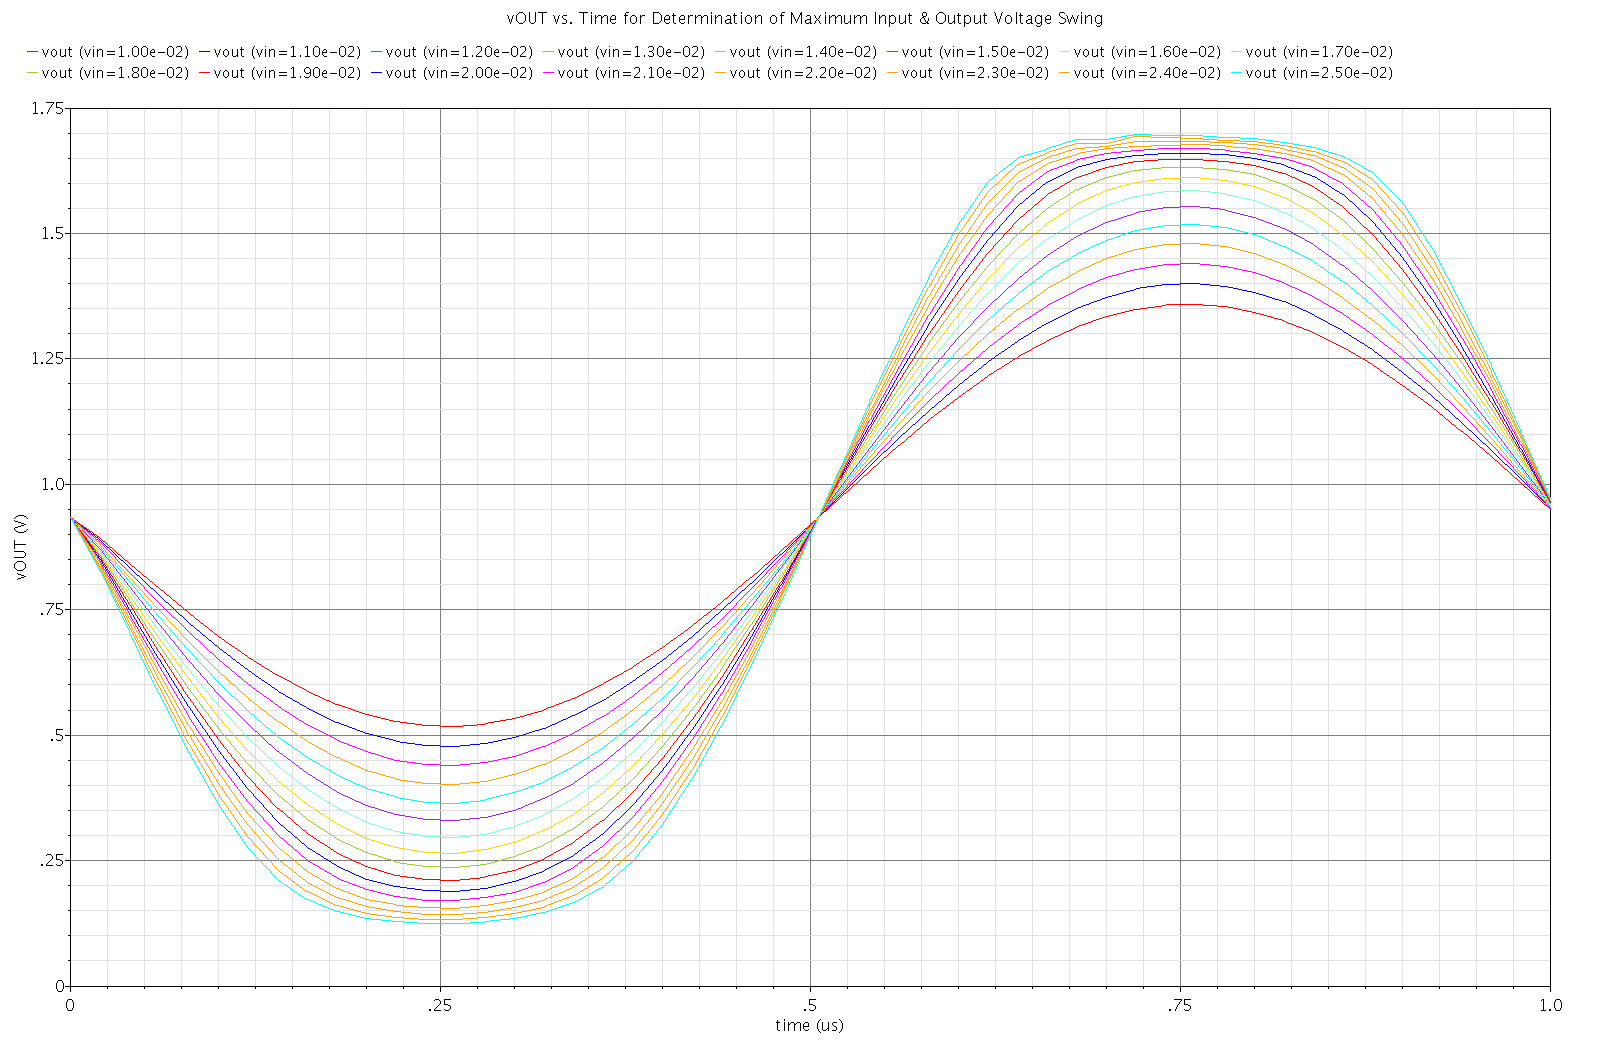
\includegraphics[width=7in]{2_cs_transient.png}
\caption{Transient Response of Output Voltage for Various Input Voltage Amplitudes}
\label{cs_tran}
\end{figure}

\begin{figure}[H]
\centering
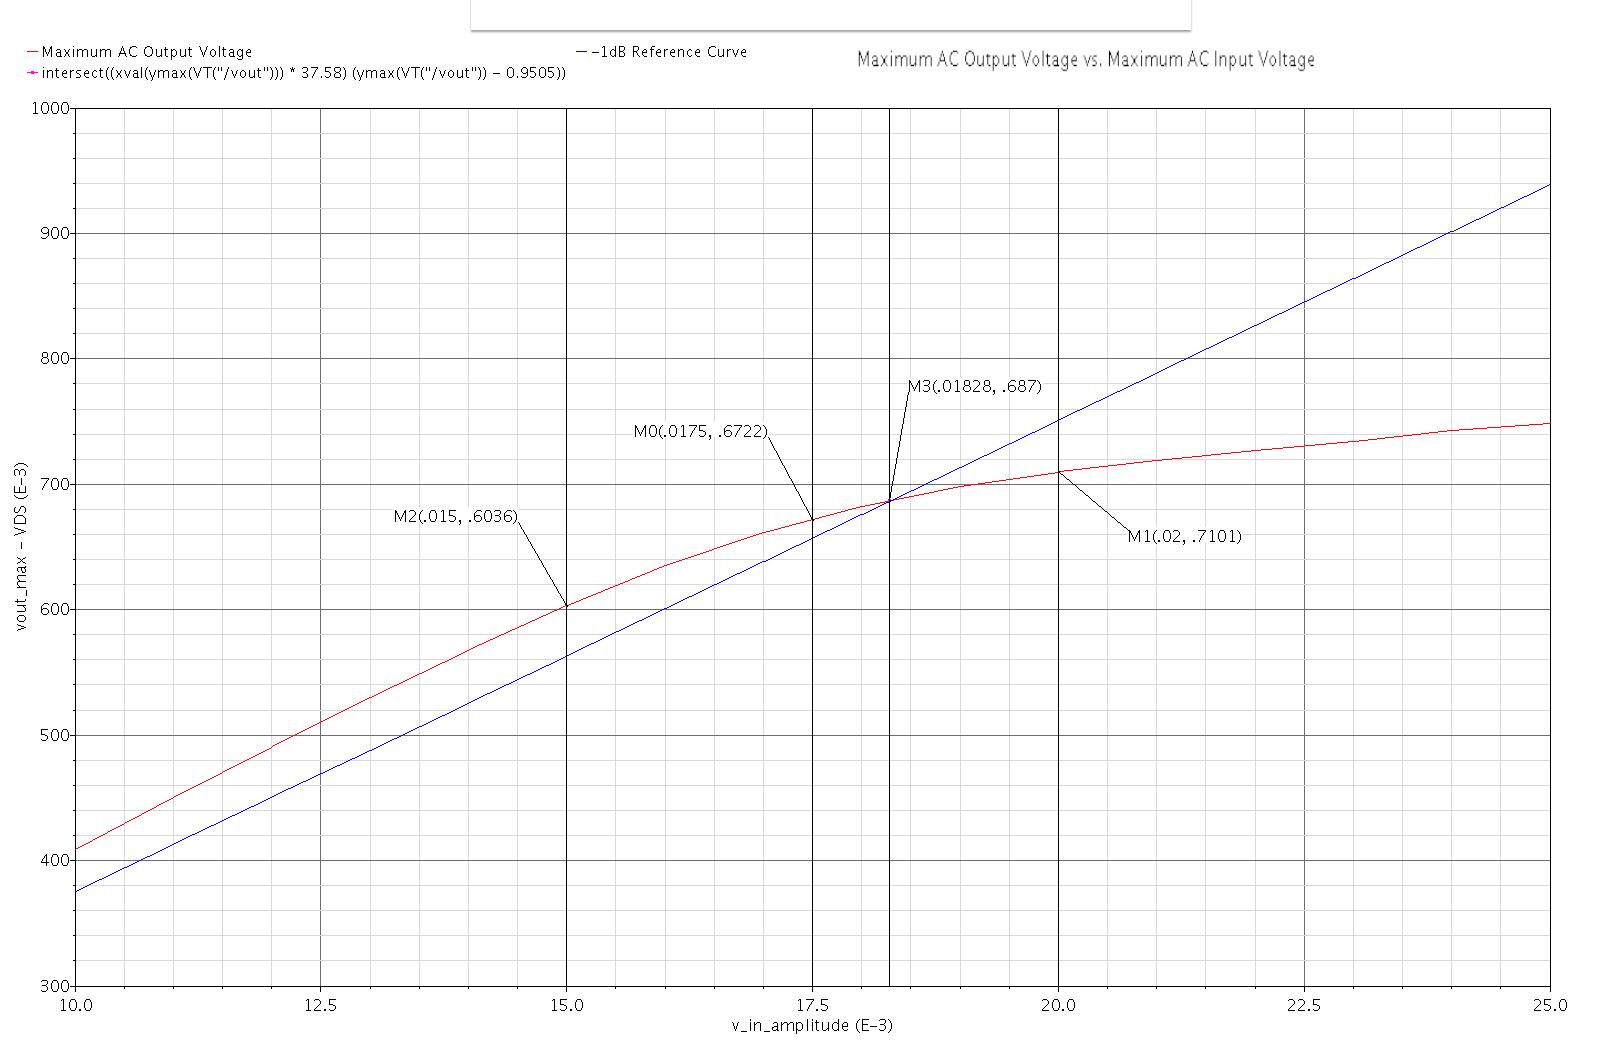
\includegraphics[width=7in]{2_cs_linearity.png}
\caption{AC Transfer Function of The Amplifier for Various Amplitudes with the -1dB Curve for Reference}
\label{cs_lin}
\end{figure}
\newpage


\subsection{Common-Drain}
I took a very similar design approach to the Common Drain amplifier as I did in the Common Source section. Because of the nature of the common drain amplifier, I knew I would only need to use one nMOS current mirror as a current source and one nMOS device for gate biasing. I began by placing both my sized amplifier device as well as unsized biasing devices. Similar to the previous design, my first goal was to maximize output voltage swing in the typical case so I aimed to achieve $V_{DS} = 900mV$ across my amplifier device. By sizing my current mirror devices appropriately, I was able to achieve a DC output voltage of 903.7mV. I then set out to set my amplifier in strong inversion to acquire maximum gain. To do this, I adjusted the sizing of transistor M11 (in Figure \ref{cd_schem} until I brought the amplifier to $V_{GS} = 566.4mV$. As a result of my biasing, the current across my amplifier device was $I_{DS} = 15.2\mu A$ which is acceptable for strong inversion. My final topology can be seen in Figure \ref{cd_schem} with annotated component parameters and Figure \ref{cd_dcop} with annotated DC operating point.

To analyze the performance of my  amplifier, I applied a small signal to the gate of my common drain. Using a 1mV input amplitude at various frequencies, I was able to achieve a gain of approximately -0.260dB in the typical case (see Figure \ref{cd_tt}). In the best case, my gain was -0.242dB (see Figure \ref{cd_ff}) and in the worst case, my gain was -0.296dB (see Figure \ref{cd_ss}). To analyze the maximum input and output voltages for linear performance, I applied various amplitudes of input voltage at 10MHz and plotted the transient output voltage. As can be seen in Figure \ref{cd_tran}, distortion begins to occur around input amplitudes of about 1V. However, because an amplitude of 1V leads to a peak-to-peak input voltage of 2V (above the power supply level), this is not a feasible value. Therefore, it can be inferred that the swing is limited by the DC input voltage of 1.469V. The maximum peak-to-peak input voltage is 0.331V and the maximum peak-to-peak output voltage is 0.321V. For reference, I compared my output voltage amplitude with the -1dB curve in Figure \ref{cd_lin}.

I calculated the gain of my circuit by hand based on the simulated values of $g_m$ and $r_o$ using the equation
\begin{equation}
a = \frac{1}{1+\frac{1}{g_mr_{o0}}+\frac{1}{g_mr_{08}}}.
\end{equation}
The result of my hand calculation was $a = 0.97\frac{V}{V}$ or in decibels $a = -0.23dB$. This is a comparable value to my simulated gain.


\begin{figure}[H]
\centering
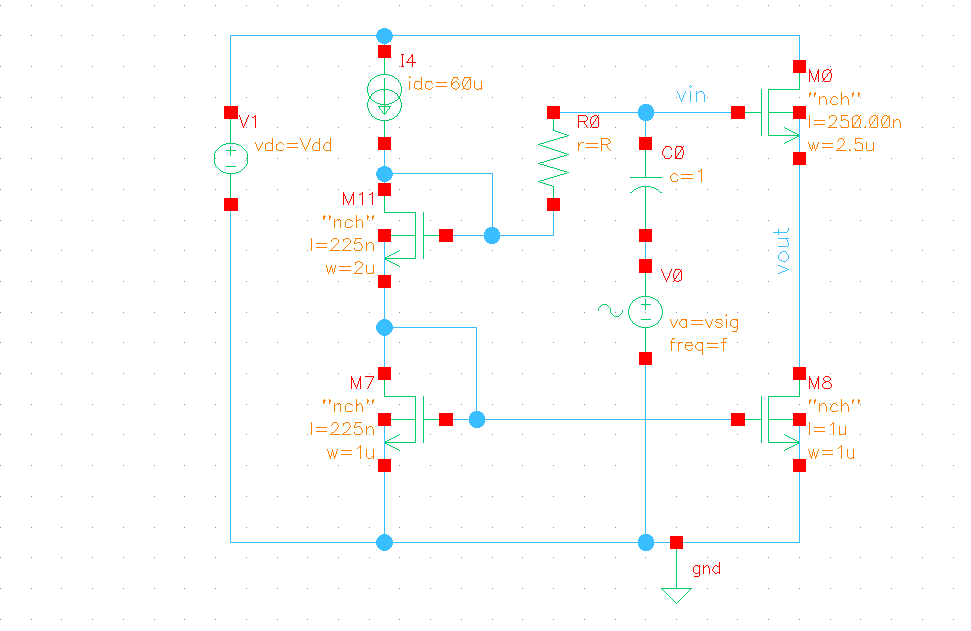
\includegraphics[width=7in]{2_cd_schematic.png}
\caption{Schematic of Common Drain Amplifier and Associated Biasing Circuitry}
\label{cd_schem}
\end{figure}

\begin{figure}[H]
\centering
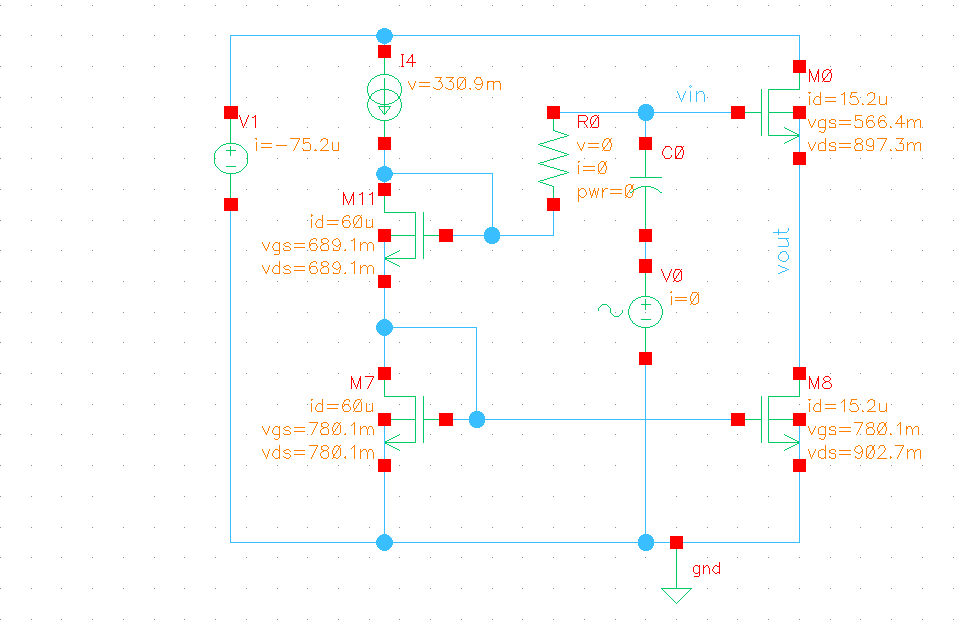
\includegraphics[width=7in]{2_cd_dcop.png}
\caption{Schematic of Common Drain Amplifier with DC Operating Point Annotations}
\label{cd_dcop}
\end{figure}

\begin{figure}[H]
\centering
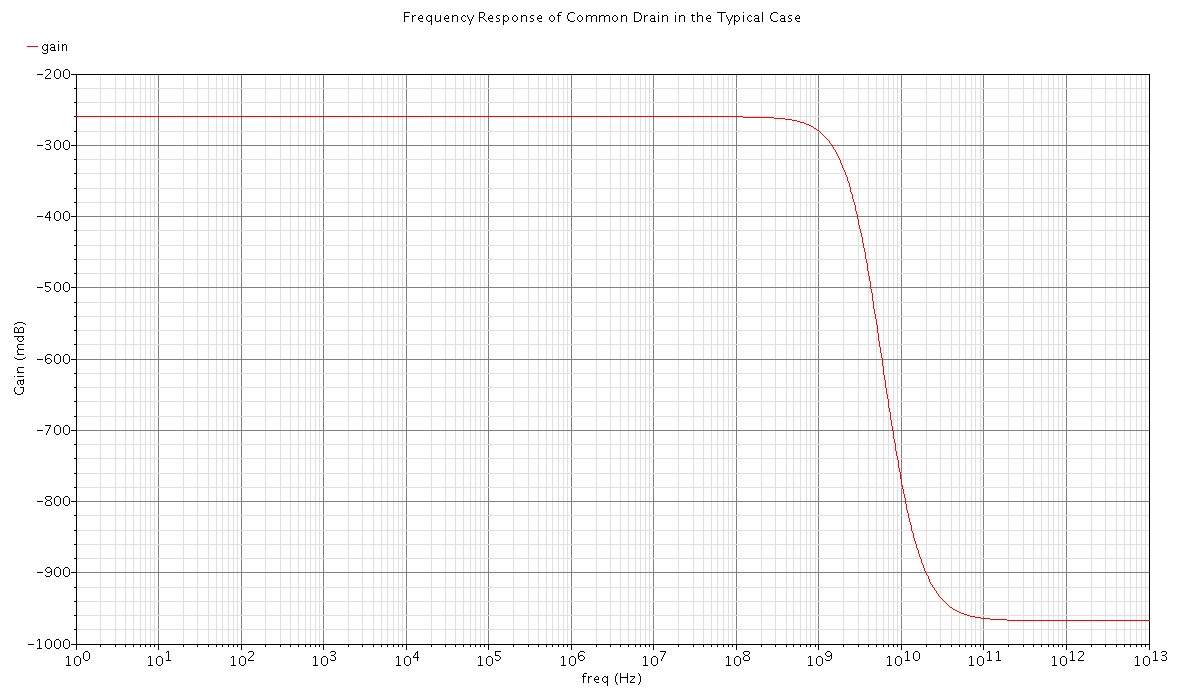
\includegraphics[width=5in]{2_cd_gain_tt.png}
\caption{Frequency Gain of Common Drain Amplifier in the Typical Case}
\label{cd_tt}
\end{figure}

\begin{figure}[H]
\centering
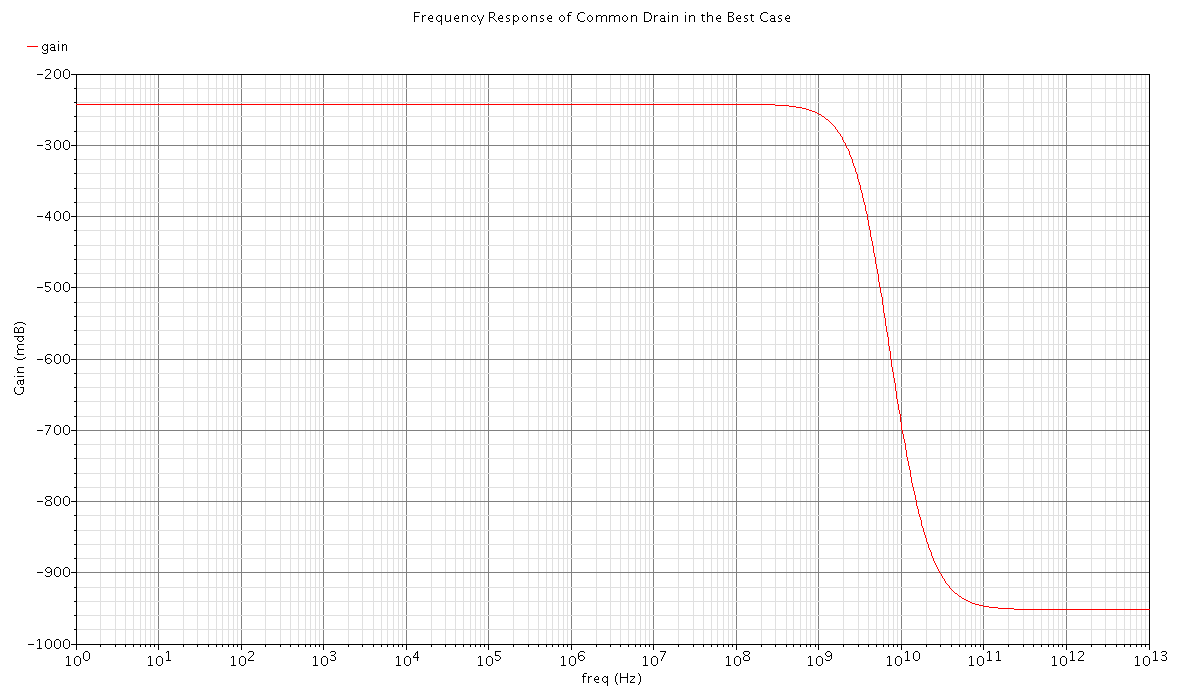
\includegraphics[width=6in]{2_cd_gain_ff.png}
\caption{Frequency Gain of Common Drain Amplifier in the Best Case}
\label{cd_ff}
\end{figure}

\begin{figure}[H]
\centering
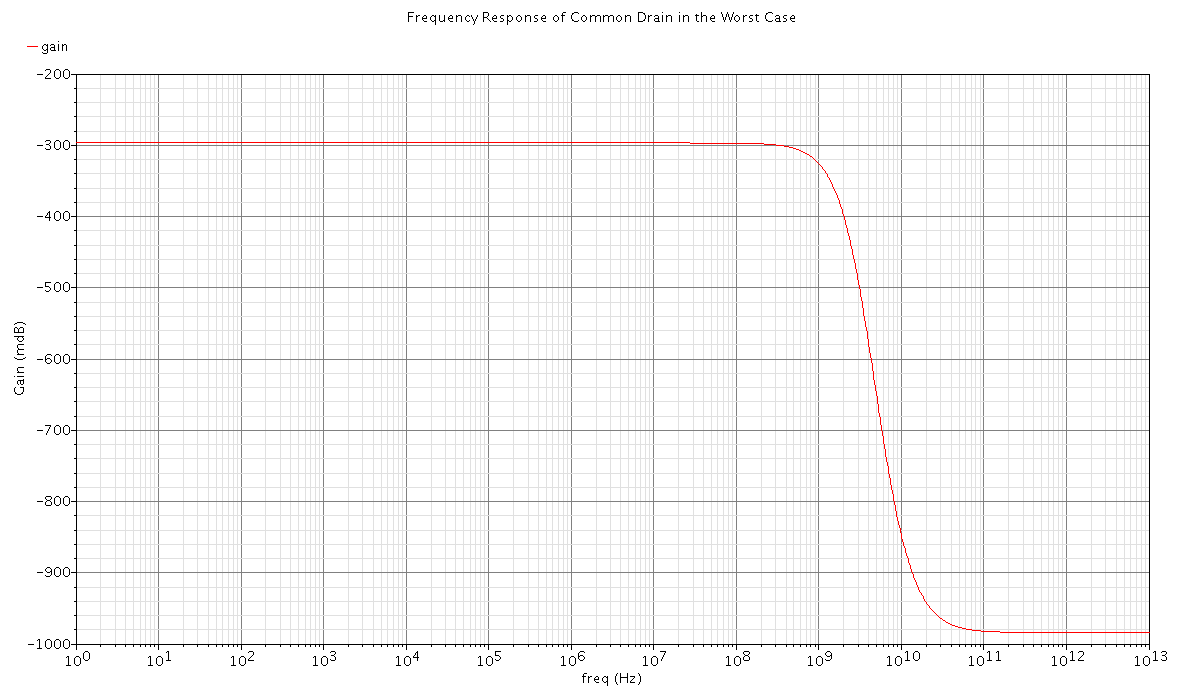
\includegraphics[width=6in]{2_cd_gain_ss.png}
\caption{Frequency Gain of Common Drain Amplifier in the Worst Case}
\label{cd_ss}
\end{figure}

\begin{figure}[H]
\centering
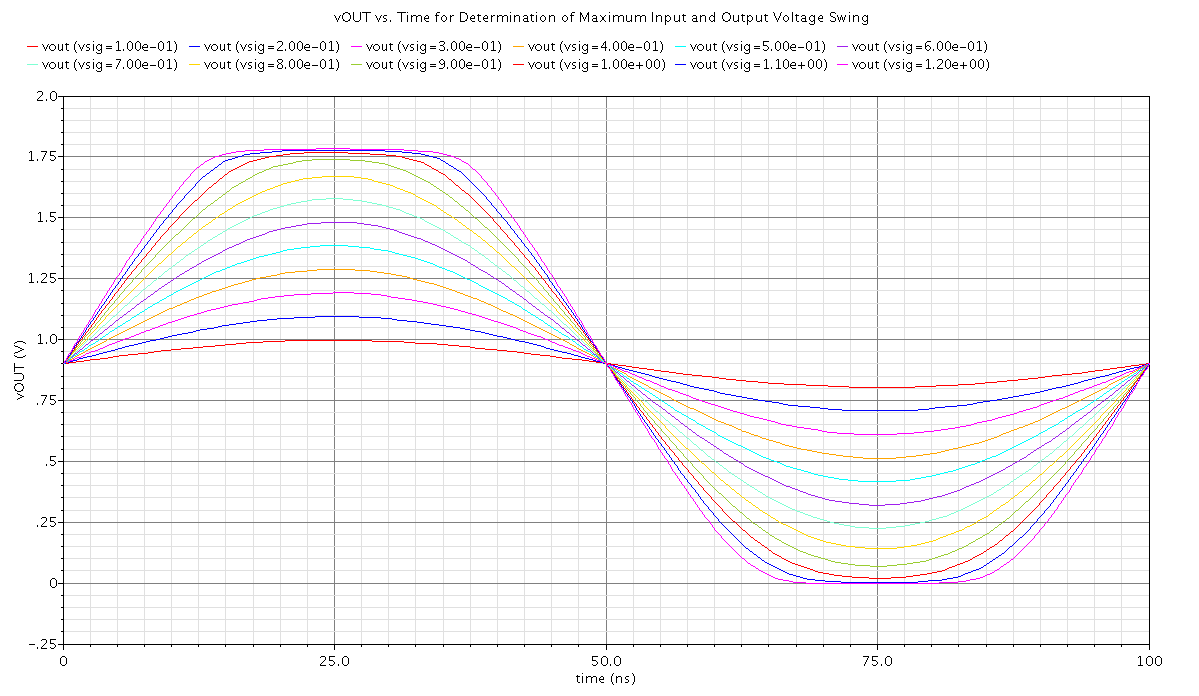
\includegraphics[width=6in]{2_cd_transient.png}
\caption{Transient Response of Output Voltage for Various Input Voltage Amplitudes}
\label{cd_tran}
\end{figure}

\begin{figure}[H]
\centering
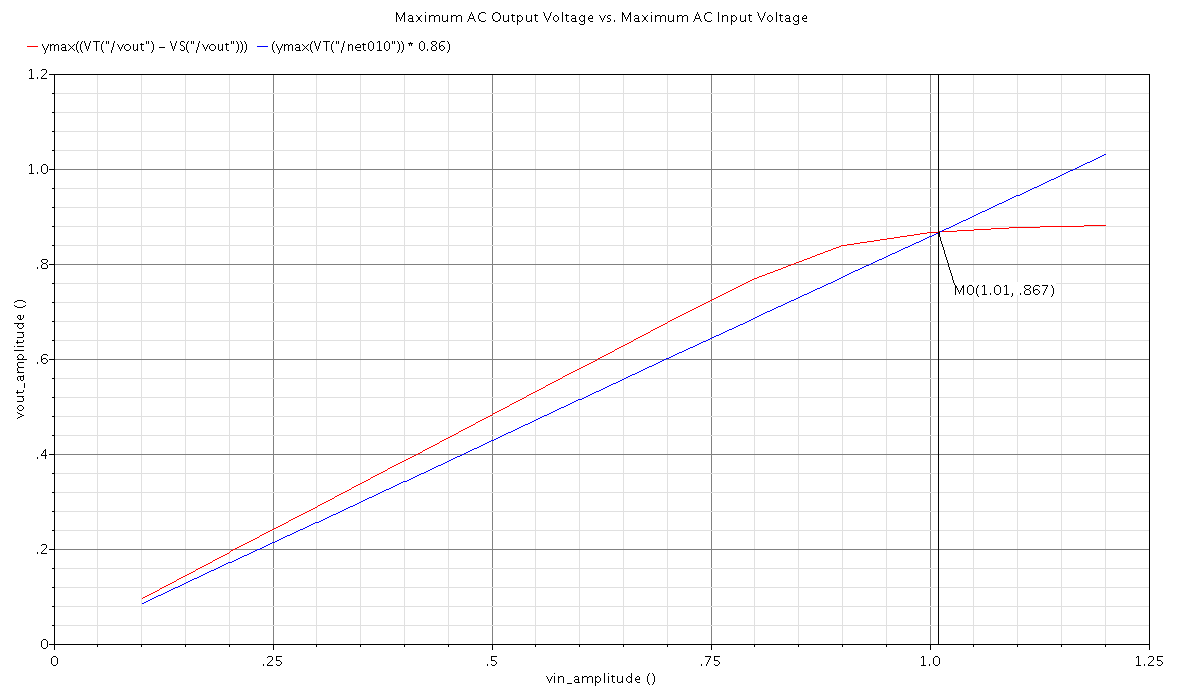
\includegraphics[width=6in]{2_cd_linearity.png}
\caption{AC Transfer Function of The Amplifier for Various Amplitudes with the -1dB Curve for Reference}
\label{cd_lin}
\end{figure}
\newpage


\subsection{Cascode}
Because the cascade amplifier includes a common source device in its topology, I began this design by placing my design from the common source amplifier of this same problem. With my already-biased common source in place, I added the top transistor of my cascade. I knew that I  had to add another branch of my bias circuit to provide voltage to the gate of this new transistor so I altered my topology (see Figure \ref{cas_schem}). With my new topology in place, I first sized the devices to achieve a DC output voltage of 0.862V. This allowed for maximum output voltage swing in the typical case. With this voltage set, and a current of $I_{DS} = 14.93\mu A$ biasing my cascade devices (appropriate for strong inversion), I had to set the correct gate voltages on each transistor for strong inversion (maximum gain). To do this, I performed a number of parametric simulations of the sizing of transistors M4 and M7. With this new data, I was able to easily find the optimal sizing, leading to $V_{GS-TOP} = 578.9mV$ and $V_{GS-BOTTOM} = 570.7mV$. My final topology can be seen in Figure \ref{cas_schem} with annotated component parameters and Figure \ref{cas_dcop} with annotated DC operating point.

To analyze the performance of my  amplifier, I applied a small signal to the gate of my common source (bottom) device. Using a 1mV input amplitude at various frequencies, I was able to achieve a gain of approximately 47.17dB in the typical case (see Figure \ref{cas_tt}). In the best case, my gain was 39.66dB (see Figure \ref{cas_ff}) and in the worst case, my gain was 38.61dB (see Figure \ref{cas_ss}). To analyze the maximum input and output voltages for linear performance, I applied various amplitudes of input voltage at 1MHz and plotted the transient output voltage. As can be seen in Figure \ref{cas_tran}, distortion begins to occur at very low voltages. This is due to the fact that the top cascade transistor is operating at a very low value of $V_{DS} = 245.1mV$ which was necessary to keep the amplifier in saturation for the best and worst case corners. When the output swings low enough, the top transistor falls out of saturation, depleting my gain. The maximum peak-to-peak input voltage is 2.44mV and the maximum peak-to-peak output voltage is 0.49mV. This was measured by comparing my output voltage amplitude with the -1dB curve shown in Figure \ref{cas_lin}.

I calculated the gain of my circuit by hand based on the simulated values of $g_m$ and $r_o$ using the equation
\begin{equation}
a = g_{m0}(r_{o2} || (r_{o0}+r_{o9}+g_{m9}r_{o0}r_{o9})).
\end{equation}
The result of my hand calculation was $a = 235.43\frac{V}{V}$ or in decibels $a = 47.42dB$. This is a comparable value to my simulated gain.


\begin{figure}[H]
\centering
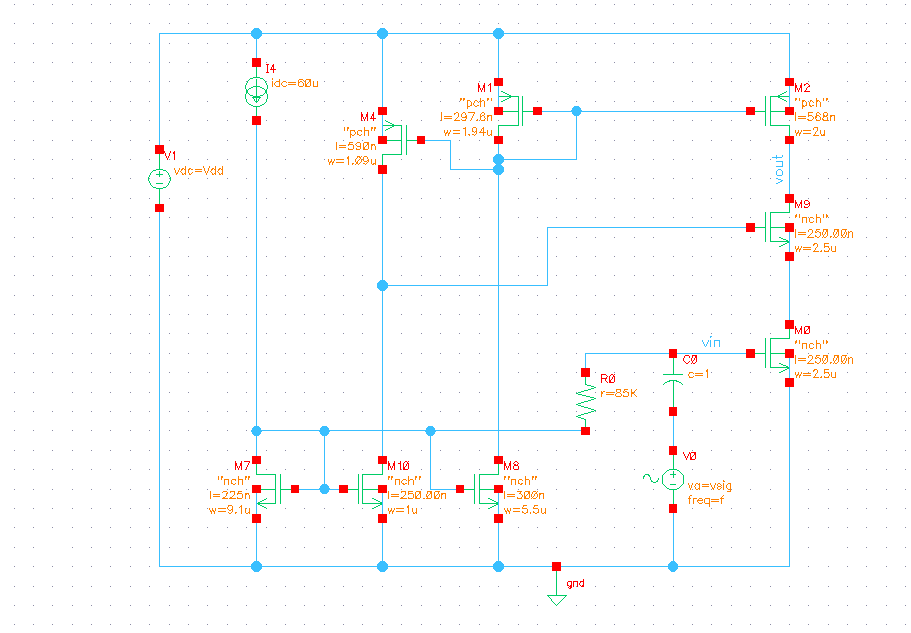
\includegraphics[width=6in]{2_cas_schematic.png}
\caption{Schematic of Cascode Amplifier and Associated Biasing Circuitry}
\label{cas_schem}
\end{figure}

\begin{figure}[H]
\centering
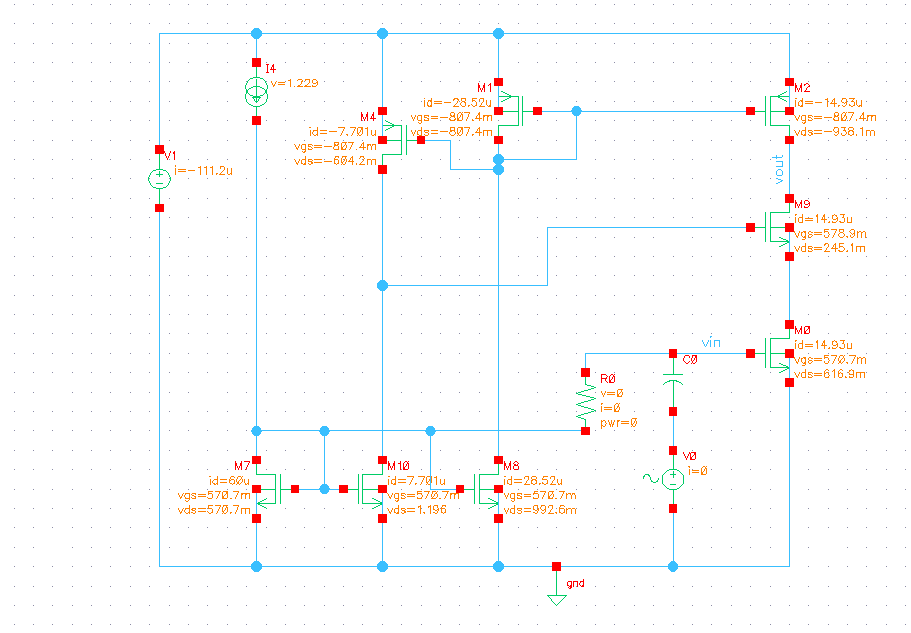
\includegraphics[width=7in]{2_cas_dcop.png}
\caption{Schematic of Cascode Amplifier with DC Operating Point Annotations}
\label{cas_dcop}
\end{figure}

\begin{figure}[H]
\centering
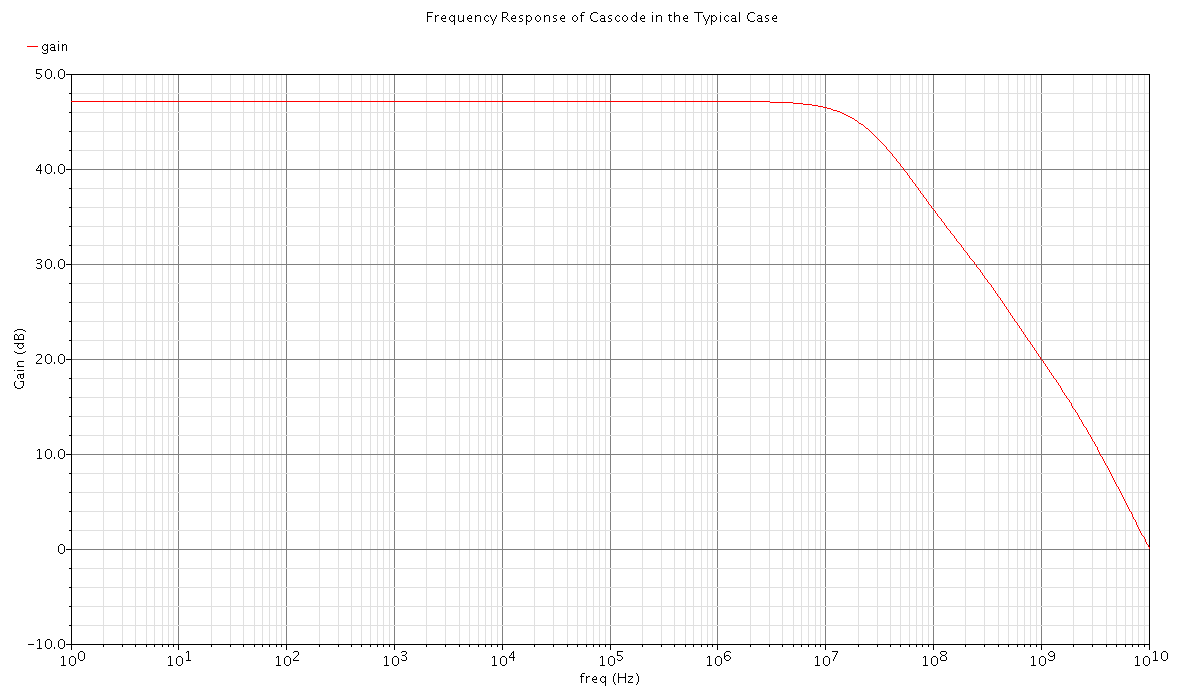
\includegraphics[width=5in]{2_cas_gain_tt.png}
\caption{Frequency Gain of Cascode Amplifier in the Typical Case}
\label{cas_tt}
\end{figure}

\begin{figure}[H]
\centering
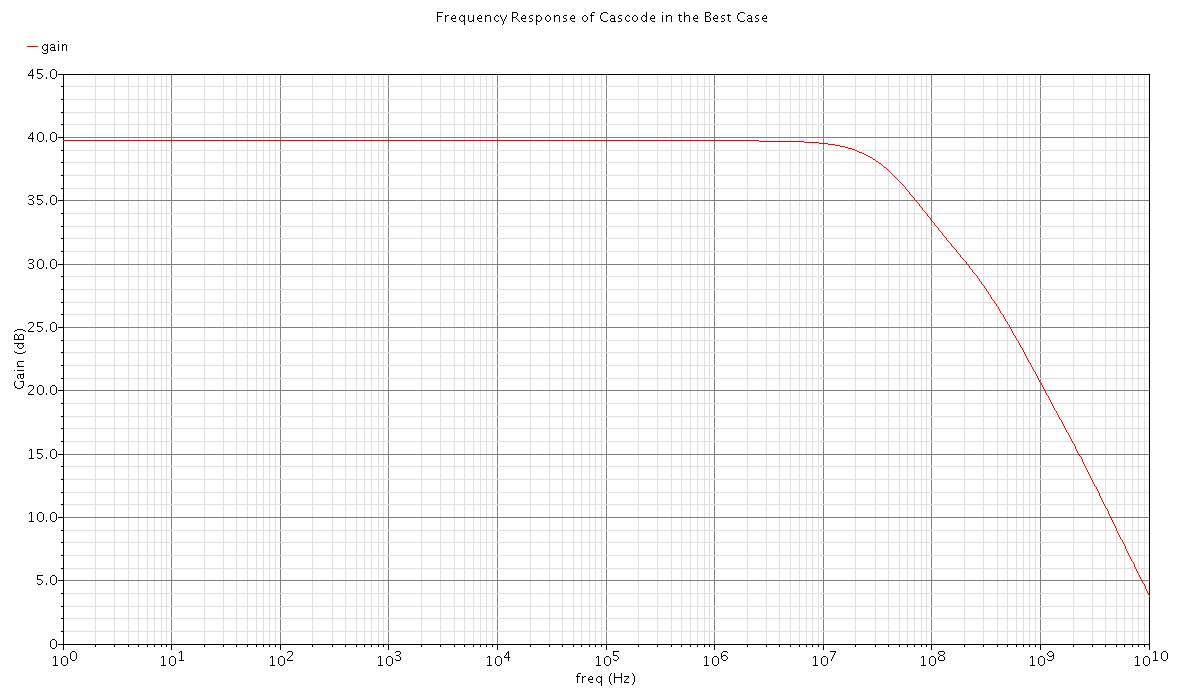
\includegraphics[width=6in]{2_cas_gain_ff.png}
\caption{Frequency Gain of Cascode Amplifier in the Best Case}
\label{cas_ff}
\end{figure}

\begin{figure}[H]
\centering
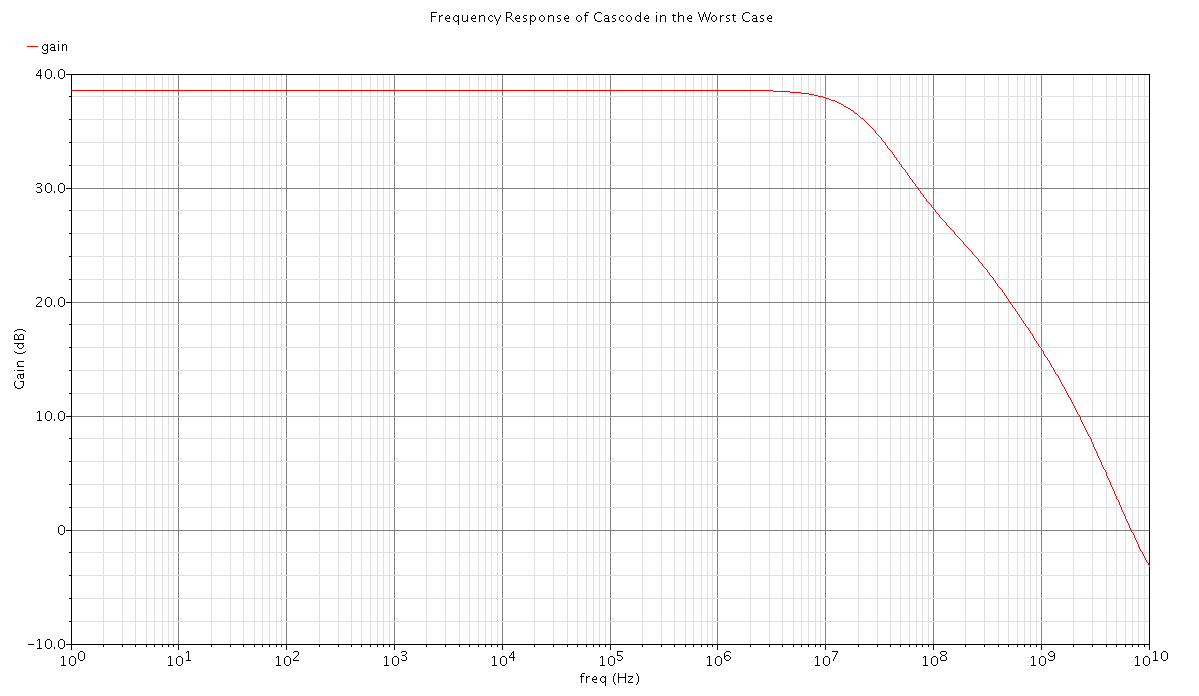
\includegraphics[width=6in]{2_cas_gain_ss.png}
\caption{Frequency Gain of Cascode Amplifier in the Worst Case}
\label{cas_ss}
\end{figure}

\begin{figure}[H]
\centering
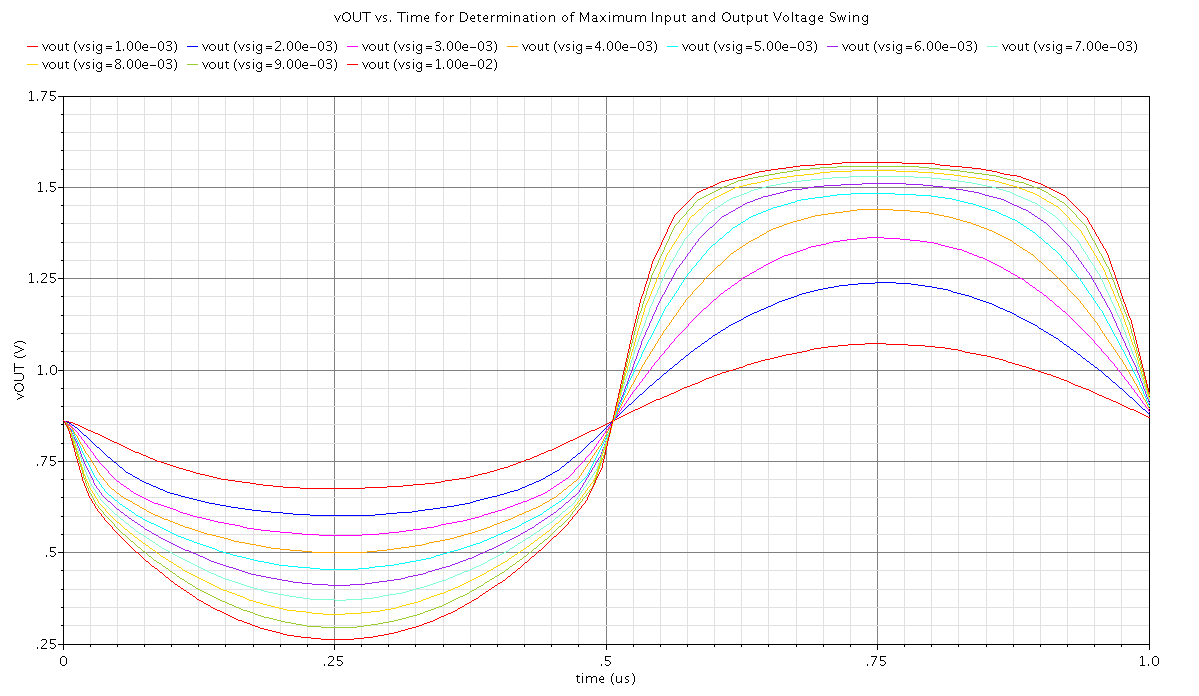
\includegraphics[width=6in]{2_cas_transient.png}
\caption{Transient Response of Output Voltage for Various Input Voltage Amplitudes}
\label{cas_tran}
\end{figure}

\begin{figure}[H]
\centering
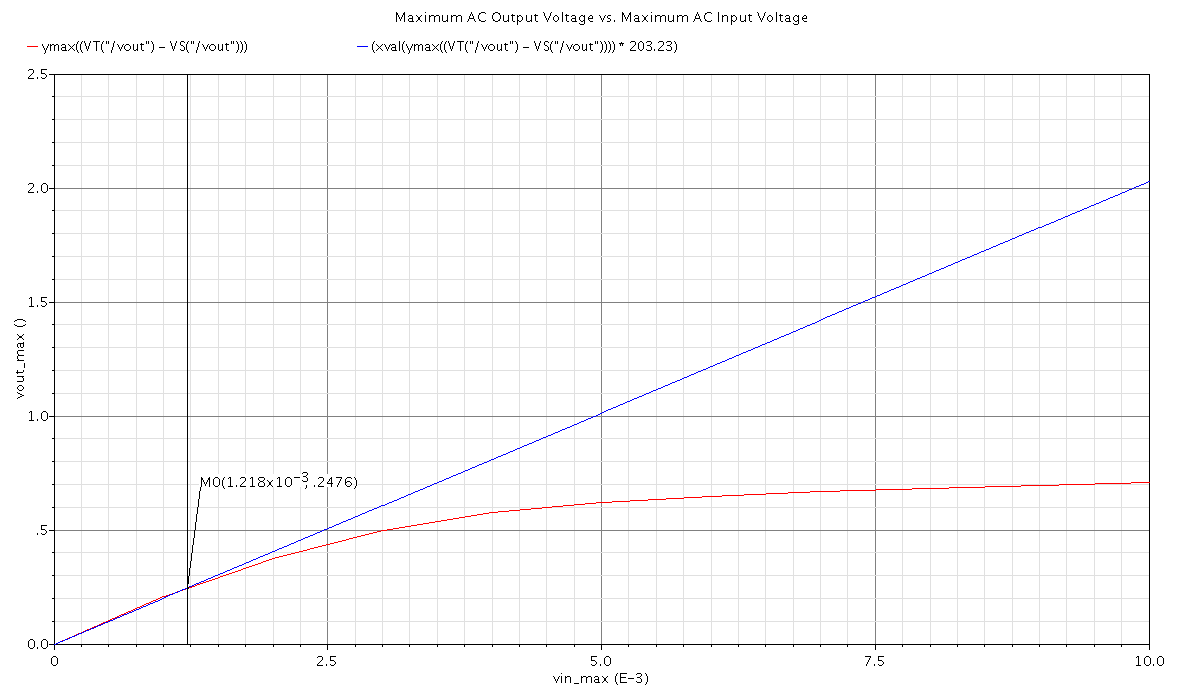
\includegraphics[width=6in]{2_cas_linearity.png}
\caption{AC Transfer Function of The Amplifier for Various Amplitudes with the -1dB Curve for Reference}
\label{cas_lin}
\end{figure}
\newpage


\end{document}
